\subsection{FOURIER TRANSFORMS OF INTEGRABLE FUNCTIONS}

In this number, we recall some definitions and results from Spectral Theories \(^{6}\) .

Denote by \(\hat{\mathbf{G}}\) the set of classes of irreducible representations of \(\mathbf{G}\) (on finite dimensional complex vector spaces). For all \(u\in \hat{\mathbf{G}}\) , denote by \(\mathrm{E}_u\) the space of \(u\) and \(d(u)\) its dimension. There exist separating positive hermitian forms on \(\mathrm{E}_u\) invariant under \(u\) , and any two such forms are proportional. Denote by \(\mathrm{A}^*\) (resp. \(\| \mathrm{A}\|_{\infty}\) ) the adjoint (resp. the norm) of an element \(\mathrm{A}\) of \(\operatorname {End}(\mathrm{E}_u)\) relative to one of these forms; for all \(g\in \mathbf{G}\) , we have \(u(g)^{*} = u(g)^{-1} = u(g^{-1})\) and \(\| u(g)\|_{\infty} = 1\) ; for all \(x\in \mathfrak{g}\) , we have \(u(x)^{*} = -u(x) = u(-x)\) .

Give \(\operatorname{End}(\mathbf{E}_u)\) the Hilbert space structure for which the scalar product is

\[
\langle \mathrm{A} | \mathrm{B} \rangle = d (u) \mathrm{Tr} (\mathrm{A} ^ {*} \mathrm{B}) = d (u) \mathrm{Tr} (\mathrm{BA} ^ {*}),\tag{1}
\]

and put

\[
\| \mathrm{A} \| _ {2} = \langle \mathrm{A} | \mathrm{A} \rangle^ {1 / 2} = (d (u) \mathrm{Tr} (\mathrm{A} ^ {*} \mathrm{A})) ^ {1 / 2}.\tag{2}
\]

We have

\[
\sqrt {d (u)} \| \mathrm{A} \| _ {\infty} \leq \| \mathrm{A} \| _ {2} \leq d (u) \| \mathrm{A} \| _ {\infty},\tag{3}
\]

SO

\[
| \langle \mathrm{A} | \mathrm{B} \rangle | \leq d (u) ^ {2} \| \mathrm{A} \| _ {\infty} \| \mathrm{B} \| _ {\infty}.\tag{4}
\]

For all \(g \in \mathrm{G}\) , we have \(\| u(g) \|_2 = d(u)\) .

Denote by \(\mathrm{F}(\hat{\mathrm{G}})\) the algebra \(\prod_{u\in \hat{\mathrm{G}}}\mathrm{End}(\mathrm{E}_u)\) . Denote by \(\mathrm{L}^2 (\hat{\mathrm{G}})\) the Hilbert sum of the Hilbert spaces \(\mathrm{End}(\mathrm{E}_u)\) ; this is the space of families \(\mathrm{A} = (\mathrm{A}_u)\in \mathrm{F}(\hat{\mathrm{G}})\) such that \(\sum_{u}\| \mathrm{A}_{u}\|_{2}^{2} < \infty\) , with the scalar product

\[
\langle \mathrm{A} | \mathrm{B} \rangle = \sum_ {u \in \hat {\mathrm{G}}} \langle \mathrm{A} _ {u} | \mathrm{B} _ {u} \rangle = \sum_ {u \in \hat {\mathrm{G}}} d (u) \operatorname{Tr} (\mathrm{A} _ {u} ^ {*} \mathrm{B} _ {u}).\tag{5}
\]

Denote the Hilbert norm on \(L^{2}(\hat{G})\) also by \(\parallel\parallel_{2}\) , so that \(\|A\|_{2}^{2}=\sum_{u\in\hat{G}}\|A_{u}\|_{2}^{2}\) for \(A\in L^{2}(\hat{G})\) .

If \(f\) is an integrable complex function on \(G\) , put

\[
u (f) = \int_ {\mathrm{G}} f (g) u (g) d g \in \operatorname{End} (\mathrm{E} _ {u})\tag{6}
\]

for all \(u \in \hat{\mathbf{G}}\) . We have \(\| u(f) \|_{\infty} \leq \int_{\mathbf{G}} |f(g)| dg = \| f \|_1\) . The Fourier cotransform of \(f\) , denoted by \(\overline{\mathcal{F}}(f)\) , is the family \((u(f))_{u \in \hat{\mathbf{G}}} \in \mathrm{F}(\hat{\mathbf{G}})\) . If \(f \in \mathrm{L}^2(\hat{\mathbf{G}})\) ,

\[
\| f \| _ {2} ^ {2} = \sum_ {u \in \hat {\mathsf {G}}} \langle u (f) | u (f) \rangle = \| \overline {{\mathcal {F}}} (f) \| _ {2} ^ {2},
\]

so \(\overline{F}\) induces an isometric linear map from the Hilbert space \(\mathrm{L}^{2}(\mathrm{G})\) to the Hilbert space \(\mathrm{L}^{2}(\hat{\mathrm{G}})\) : in other words, for f and \(f'\) in \(\mathrm{L}^{2}(\mathrm{G})\) , we have

\[
\int_ {\mathrm{G}} \overline {{f (g)}} f ^ {\prime} (g) d g = \langle \overline {{\mathcal {F}}} (f) | \overline {{\mathcal {F}}} (f ^ {\prime}) \rangle = \sum_ {u \in \hat {\mathrm{G}}} d (u) \mathrm{Tr} (u (f) ^ {*} u (f ^ {\prime})).\tag{7}
\]

For \(f\) and \(f'\) in \(\mathrm{L}^1(\mathrm{G})\) , the convolution product \(f * f'\) of \(f\) and \(f'\) is defined by

\[
(f * f ^ {\prime}) (h) = \int_ {G} f (h g ^ {- 1}) f ^ {\prime} (g) d g = \int_ {G} f (g) f ^ {\prime} (g ^ {- 1} h) d g
\]

(the integral makes sense for almost all \(h \in \mathbf{G}\) ).

We have \(f * f' \in L^{1}(G)\) and, for all \(u \in \hat{G}\) , \(u(f * f') = u(f)u(f')\) , so

\[
\overline {{{{\mathcal {F}}}}} (f * f ^ {\prime}) = \overline {{{{\mathcal {F}}}}} (f). \overline {{{{\mathcal {F}}}}} (f ^ {\prime}).\tag{8}
\]

Conversely, let \(\mathrm{A} = (\mathrm{A}_{u})_{u \in \hat{\mathrm{G}}}\) be an element of \(\mathrm{F}(\hat{\mathrm{G}})\) ; for all \(u \in \hat{G}\) , let \(F_{u}A\) be the (analytic) function on G defined by

\[
(\mathcal {F} _ {u} \mathrm{A}) (g) = \langle u (g) | \mathrm{A} _ {u} \rangle = d (u) \mathrm{Tr} (\mathrm{A} _ {u} u (g) ^ {- 1}).\tag{9}
\]

If \(\mathrm{A} \in \mathrm{L}^2(\hat{\mathrm{G}})\) , the family \((\mathcal{F}_u\mathrm{A})_{u \in \hat{\mathrm{G}}}\) is summable in \(\mathrm{L}^2(\mathrm{G})\) ; the Fourier transform of \(\mathrm{A}\) , denoted by \(\mathcal{F}(\mathrm{A})\) , is the sum of this family. The maps \(\overline{\mathcal{F}}\) and \(\mathcal{F}\) are inverse isomorphisms between the Hilbert spaces \(\mathrm{L}^2(\mathrm{G})\) and \(\mathrm{L}^2(\hat{\mathrm{G}})\) .

In other words:

PROPOSITION 1. Every square integrable complex function \(f\) on \(G\) is the sum in the Hilbert space \(L^2(G)\) of the family \((f_u)_{u\in \hat{G}}\) where, for all \(h\in G\) and all \(u\in \hat{G}\) ,

\[
\begin{array}{l} f _ {u} (h) = \langle u (h) | u (f) \rangle \\ \qquad = d (u) \int_ {\mathrm{G}} f (g) \mathrm{Tr} (u (g h ^ {- 1}))   d g = d (u) \int_ {\mathrm{G}} f (g h) \mathrm{Tr} (u (g))   d g. \end{array}\tag{10}
\]

For all \(u \in \hat{\mathrm{G}}\) choose an orthonormal basis \(\mathrm{B}_u\) of \(\mathrm{E}_u\) , and denote by \((u_{ij}(g))\) the matrix of \(u(g)\) in this basis. Prop. 1 also means that the family of functions \(\sqrt{d(u)} u_{ij}\) , for \(u\) in \(\hat{\mathrm{G}}\) and \(i,j\) in \(\mathrm{B}_u\) , is an orthonormal basis of the space \(\mathrm{L}^2 (\mathrm{G})\) .

If f is an integrable function on G such that the family \((f_{u})\) is uniformly summable, then the sum of this family is a continuous function which coincides almost everywhere with f; in other words, if we assume in addition that f is continuous, then for all \(h \in G\) ,

\[
f (h) = \sum_ {u \in \hat {\mathrm{G}}} d (u) \int_ {\mathrm{G}} f (g h) \mathrm{Tr} (u (g))   d g.\tag{11}
\]

Conversely, let \(\mathrm{A} \in \mathrm{F}(\hat{\mathrm{G}})\) ; if the family \((\mathcal{F}_u\mathrm{A})_{u \in \hat{\mathrm{G}}}\) is uniformly summable, the function

\[
g \mapsto \sum_ {u \in \hat {\mathrm{G}}} (\mathcal {F} _ {u} \mathrm{A}) (g) = \sum_ {u \in \hat {\mathrm{G}}} d (u) \mathrm{Tr} (\mathrm{A} _ {u} u (g) ^ {- 1})
\]

is a continuous function on \(G\) whose Fourier cotransform is \(A\) .

Let \(f\) be an integrable function on \(\mathbf{G}\) , and let \(s \in \mathbf{G}\) . Denote by \(\gamma(s)f\) and \(\delta(s)f\) the functions on \(\mathbf{G}\) defined by \(\gamma(s)f = \varepsilon_s * f\) , \(\delta(s)f = f * \varepsilon_{s^{-1}}\) , that is,

\[
(\gamma (s) f) (g) = f (s ^ {- 1} g), \quad (\delta (s) f) (g) = f (g s) \text { for } g \in \mathrm{G},
\]

(Chap. III, §3, no. 4 and Integration, Chap. VII, §1, no. 1). We have

\[
u (\gamma (s) f) = \int_ {\mathrm{G}} f (s ^ {- 1} g) u (g) d g = \int_ {\mathrm{G}} f (g) u (s g) d g,
\]

SO

\[
u (\gamma (s) f) = u (s) u (f),\tag{12}
\]

and similarly

\[
u (\delta (s ^ {- 1}) f) = u (f) u (s).\tag{13}
\]

When G is commutative, \(\hat{G}\) is the underlying set of the dual group of G (Spectral Theories, Chap. II, §1, no. 1), \(d(u) = 1\) for all \(u \in \hat{G}\) , and we recover the definitions of the Fourier transform given in Spectral Theories, Chap. II.

\subsection{FOURIER TRANSFORMS OF INFINITELY-DIFFERENTIABLE FUNCTIONS}

Recall (Chap. III, §3, no. 1, Def. 2) that U(G) denotes the algebra of distributions on G with support contained in \(\{e\}\) . The canonical injection of g into U(G) extends to an isomorphism from the enveloping algebra of the Lie algebra g to U(G) (loc. cit., no. 7, Prop. 25); from now on we identify these two algebras by this isomorphism. If f is an infinitely-differentiable complex function on G and if \(t \in \mathrm{U}(\mathrm{G})\) , we denote by \(L_{t}f\) and \(R_{t}f\) the functions on G defined by

\[
\mathrm{L} _ {t} f (g) = \langle \varepsilon_ {g} * t, f \rangle , \quad \mathrm{R} _ {t} f (g) = \langle t * \varepsilon_ {g}, f \rangle
\]

(cf.~loc. cit., no. 6). For all \(g \in G\) ,

\[
\mathrm{L} _ {t} \circ \gamma (g) = \gamma (g) \circ \mathrm{L} _ {t}, \quad \mathrm{R} _ {t} \circ \delta (g) = \delta (g) \circ \mathrm{R} _ {t}.
\]

Let \(u \in \hat{G}\) ; denote by \(E_u\) the space of \(u\) . The morphism of Lie groups \(u: G \to \mathbf{GL}(E_u)\) gives by differentiation a homomorphism of (real) Lie algebras \(\mathfrak{g} \to \text{End}(E_u)\) , hence a homomorphism of algebras, also denoted by \(u\) , from \(U(G)\) to \(\text{End}(E_u)\) . If \(t \in U(G)\) and if \(f\) is an infinitely-differentiable function on \(G\) , then

\[
u (\mathrm{L} _ {t} f) = u (f) u (t ^ {\vee}), \quad u (\mathrm{R} _ {t} f) = u (t ^ {\vee}) u (f),\tag{14}
\]

where \(t^{\vee}\) denotes the image of t under the principal anti-automorphism of U(G) (Chap. I, §2, no. 4); indeed, it suffices to verify this for \(t \in g\) , in which case it follows by differentiation from formulas (12) and (13) (cf.~Chap. III, §3, no. 7, Prop. 27).

For all \(u \in \hat{\mathbf{G}}\) , denote by \(\lambda(u)\) the highest weight of \(u\) (§7, no. 2, Th. 1), so \(u \mapsto \lambda(u)\) is a bijective map from \(\hat{\mathbf{G}}\) to the set \(\mathrm{X}_{++}\) of dominant elements of \(\mathrm{X}(\mathrm{T})\) .

Let \(\Gamma \in \mathrm{U}(\mathrm{G})\) be a Casimir element of \(\mathrm{G}\) (§7, no. 6); for all \(u \in \hat{\mathrm{G}}\) , the endomorphism \(u(\Gamma)\) of \(\mathrm{E}_u\) is a homothety, whose ratio we denote by \(\tilde{\Gamma}(u)\) , so we have a map \(u \mapsto \tilde{\Gamma}(u)\) from \(\hat{\mathrm{G}}\) to \(\mathbf{C}\) .

If \(\varphi\) and \(\psi\) are two functions on \(\hat{G}\) with positive real values, denote by `` \(\varphi \preccurlyeq \psi\) '' or `` \(\varphi(u) \preccurlyeq \psi(u)\) '' the relation ``there exists M \textgreater{} 0 such that \(\varphi(u) \leq M\psi(u)\) for all \(u \in \hat{G}\) ''; this is a pre-order relation on the set of functions on \(\hat{G}\) with positive real values.

PROPOSITION 2. Let \(m \mapsto \|m\|\) be a norm on the R-vector space \(\mathbf{R} \otimes \mathrm{X(T)}\) and \(\Gamma\) a Casimir element of G. Let \(\varphi\) be a function on \(\hat{\mathrm{G}}\) with positive real values.

\begin{enumerate}
\def\labelenumi{\alph{enumi})}
\tightlist
\item
  The following conditions are equivalent:
\end{enumerate}

\begin{enumerate}
\def\labelenumi{(\roman{enumi})}
\item
  There exists an integer \(n > 0\) such that \(\varphi(u) \preccurlyeq (\|\lambda(u)\| + 1)^n\) (resp. for every integer \(n > 0\) , we have \(\varphi(u) \preccurlyeq (\|\lambda(u)\| + 1)^{-n}\) ).
\item
  There exists an integer \(n > 0\) such that \(\varphi(u) \preccurlyeq (\tilde{\Gamma}(u) + 1)^n\) (resp. for every integer \(n > 0\) , we have \(\varphi(u) \preccurlyeq (\tilde{\Gamma}(u) + 1)^{-n}\) ).
\end{enumerate}

\begin{enumerate}
\def\labelenumi{\alph{enumi})}
\setcounter{enumi}{1}
\tightlist
\item
  If \(\mathrm{G}\) is semi-simple, conditions (i) and (ii) are also equivalent to:
\end{enumerate}

\begin{enumerate}
\def\labelenumi{(\roman{enumi})}
\setcounter{enumi}{2}
\tightlist
\item
  There exists an integer \(n > 0\) such that \(\varphi(u) \preccurlyeq d(u)^n\) (resp. for every integer \(n > 0\) , we have \(\varphi(u) \preccurlyeq d(u)^{-n}\) ).
\end{enumerate}

Note first of all that condition (i) is clearly independent of the choice of norm. Thus we can use the norm defined by the quadratic form \(Q_{\varGamma}\) associated to \(\varGamma\) (§7, no. 6, Prop. 4). Then

\[
0 \leq \tilde {\Gamma} (u) = \| \lambda (u) + \rho \| ^ {2} - \| \rho \| ^ {2},
\]

so \(\tilde{\Gamma}(u) + 1 \preccurlyeq (\|\lambda(u)\| + 1)^2 \preccurlyeq \tilde{\Gamma}(u) + 1\) , hence \(a\) .

Further, if G is semi-simple,

\[
\left\| \lambda (u) + \rho \right\| \preccurlyeq d (u) \preccurlyeq \left\| \lambda (u) + \rho \right\| ^ {\mathrm{N}}, \quad \text { where } \mathrm{N} = 1 / 2 (\dim \mathrm{G} - \dim \mathrm{T})
\]

(§7, no. 5, Cor. 1 of Th. 3), so \(\| \lambda(u) \| + 1 \preccurlyeq d(u) \preccurlyeq (\| \lambda(u) \| + 1)^{\mathrm{N}}\) , hence \(b\) ).

It follows from Prop. 2 that condition (i) is independent of the choice of maximal torus, chamber, and norm, and that condition (ii) is independent of the choice of Casimir element. A function \(\varphi\) satisfying conditions (i) and (ii) is said to be moderately increasing (resp. rapidly decreasing). The product of two moderately increasing functions is moderately increasing; the product of a moderately increasing function and a rapidly decreasing function is rapidly decreasing. If \(\varphi\) is rapidly decreasing, the family \((\varphi(u))_{u\in\hat{G}}\) is summable.

Examples. The function \(u \mapsto d(u)\) is moderately increasing (§7, no. 5, Cor. 1 of Th. 3); for any norm \(\| \cdot \|\) on \(\mathbf{R} \otimes \mathrm{X(T)}\) , the function \(u \mapsto \| \lambda(u) \|\) is moderately increasing. For any Casimir element \(\Gamma\) , the function \(u \mapsto \tilde{\Gamma}(u)\) is moderately increasing; more generally:

PROPOSITION 3. For all \(t \in \mathrm{U}(\mathrm{G})\) , the functions \(u \mapsto \| u(t) \|_{\infty}\) and \(u \mapsto \| u(t) \|_2\) on \(\hat{\mathrm{G}}\) are moderately increasing.

Since the product of two moderately increasing functions is moderately increasing, it suffices to prove this when \(t \in g\) : in that case the assertion follows from the Remark in §7, no. 6 and the inequality

\[
\| u (t) \| _ {2} \leq d (u) \| u (t) \| _ {\infty}.
\]

THEOREM 1. a) Let \(f\) be an infinitely-differentiable complex function on \(\mathbf{G}\) . Then the family \((f_u)_{u\in \hat{\mathbf{G}}}\) , where \(f_{u}(g) = \langle u(g)|u(f)\rangle\) , is uniformly summable on \(\mathbf{G}\) and, for all \(h\in \mathbf{G}\) ,

\[
f (h) = \sum_ {u \in \hat {\mathrm{G}}} \langle u (h) | u (f) \rangle = \sum_ {u \in \hat {\mathrm{G}}} d (u) \int_ {\mathrm{G}} f (g) \mathrm{Tr} (u (g h ^ {- 1}))   d g.
\]

\begin{enumerate}
\def\labelenumi{\alph{enumi})}
\setcounter{enumi}{1}
\tightlist
\item
  Let \(f\) be an integrable function on \(\mathbf{G}\) ; then \(f\) is equal almost everywhere to an infinitely-differentiable function if and only if the function \(u \mapsto \| u(f) \|_{\infty}\) is rapidly decreasing on \(\hat{\mathbf{G}}\) .
\end{enumerate}

Let \(f\) be an infinitely-differentiable function on \(G\) , and let \(\Gamma\) be a Casimir element for \(G\) ; by formula (14),

\[
\tilde {\Gamma} (u) ^ {n} u (f) = u (f) u (\Gamma) ^ {n} = u ((\mathrm{L} _ {\Gamma}) ^ {n} f)
\]

for all \(n \geq 0\) , and consequently

\[
\tilde {\Gamma} (u) ^ {n} \| u (f) \| _ {\infty} \leq \| (\mathrm{L} _ {\Gamma}) ^ {n} f \| _ {1} \leq \sup _ {g \in \mathrm{G}} | ((\mathrm{L} _ {\Gamma}) ^ {n} f) (g) |;\tag{15}
\]

thus, the function \(u \mapsto \|u(f)\|_{\infty}\) is indeed rapidly decreasing.

Conversely, let \(\mathrm{A} = (\mathrm{A}_{u})_{u \in \hat{\mathrm{G}}}\) be an element of \(\mathrm{F}(\hat{\mathrm{G}})\) such that the function \(u \mapsto \|A_{u}\|_{\infty}\) is rapidly decreasing. Put \(f_{u}(g) = \langle u(g)|A_{u} \rangle\) ; the function \(g \mapsto f_{u}(g)\) is analytic, hence infinitely-differentiable. By Chap. III, §3, no. 7, Prop. 27,

\[
(\mathrm{L} _ {x} f _ {u}) (g) = \langle u (g) u (x) | \mathrm{A} _ {u} \rangle
\]

for all \(x \in \mathfrak{g}\) . Let \(t \in \mathrm{U}(\mathrm{G})\) ; by the preceding formula,

\[
(\mathrm{L} _ {t} f _ {u}) (g) = \langle u (g) u (t) | \mathrm{A} _ {u} \rangle
\]

and consequently

\[
\begin{array}{r} | (\mathrm{L} _ {t} f _ {u}) (g) | = | \langle u (g) u (t) | \mathrm{A} _ {u} \rangle \leq d (u) ^ {2} \| u (t) \| _ {\infty} \| u (g) \| _ {\infty} \| \mathrm{A} _ {u} \| _ {\infty} \\ = d (u) ^ {2} \| u (t) \| _ {\infty} \| \mathrm{A} _ {u} \| _ {\infty}. \end{array}
\]

Since \(d(u)\) and \(\|u(t)\|_{\infty}\) are moderately increasing (Prop. 3) and \(\|A_{u}\|_{\infty}\) is rapidly decreasing, the function \(u \mapsto \sup_{g} |(\mathrm{L}_{t}f_{u})(g)|\) is rapidly decreasing; thus, the family \((\mathrm{L}_{t}f_{u})_{u \in \hat{\mathrm{G}}}\) is uniformly summable. It follows \(^{7}\) that the sum of the family \((f_{u})\) is an infinitely-differentiable function on G, whose Fourier cotransform is \((\mathrm{A}_{u})\) , hence the theorem.

Denote by \(\mathcal{S}(\hat{\mathrm{G}})\) the vector subspace of \(\mathrm{L}^2 (\hat{\mathrm{G}})\) consisting of the families \(\mathrm{A} = (\mathrm{A}_u)_{u\in \hat{\mathrm{G}}}\) such that the function \(u\mapsto \| \mathrm{A}_u\|_\infty\) is rapidly decreasing on \(\hat{\mathrm{G}}\) . It follows from the theorem that the maps \(\overline{\mathcal{F}}:f\mapsto (u(f))_{u\in \hat{\mathrm{G}}}\) and \(\mathcal{F}\colon \mathrm{A}\mapsto \sum_{u\in \hat{\mathrm{G}}}\langle u(g)|\mathrm{A}_u\rangle\) induce inverse isomorphisms between the complex vector spaces \(\mathcal{C}^\infty (\mathrm{G};\mathbf{C})\) and \(\mathcal{S}(\hat{\mathrm{G}})\) . Give the space \(\mathcal{C}^\infty (\mathrm{G};\mathbf{C})\) the topology of uniform \(\mathrm{C}^\infty\) -convergence (§6, no. 4) which can be defined by the family of semi-norms \(f\mapsto \sup_{g\in \mathrm{G}}|\mathrm{L}_t f(g)|\) for \(t\in \mathrm{U}(\mathrm{G})\) , and the space \(\mathcal{S}(\hat{\mathrm{G}})\) the topology defined by the sequence of semi-norms \(p_n:\mathrm{A}\mapsto \sup_{u\in \hat{\mathrm{G}}}(\tilde{\Gamma} (u) + 1)^n\| \mathrm{A}_u\|_\infty\) . Formula (15) of the preceding proof shows that \(\overline{\mathcal{F}}\) is continuous. Let \(t\in \mathrm{U}(\mathrm{G})\) , and let \(\mathrm{A} = (\mathrm{A}_u)_{u\in \hat{\mathrm{G}}}\) be an element of \(\mathcal{S}(\hat{\mathrm{G}})\) ; put \(f_{n}(g) = \langle u(g)|\mathrm{A}_{u}\rangle\) . Let \(p\) be an integer such that \(\sum_{u\in \hat{\mathrm{G}}} \tilde{\Gamma} (u)^{-p} = \mathrm{M} < \infty\) . By the preceding proof, there exists a positive integer \(m\) such that, for all \(g\in \mathrm{G}\) ,

\[
| (\mathrm{L} _ {t} f _ {u}) (g) | \leq d (u) ^ {2} \| u (t) \| _ {\infty} \| \mathrm{A} _ {u} \| _ {\infty} \leq m. (1 + \tilde {\Gamma} (u)) ^ {m} \tilde {\Gamma} (u) ^ {- p} \| \mathrm{A} _ {u} \| _ {\infty}
\]

so \(|(\mathrm{L}_t\mathcal{F}(\mathrm{A}))(g)| \leq m\mathrm{M}p_m(\mathrm{A})\) ; this proves that \(\mathcal{F}\) is continuous. Consequently:

COROLLARY. The maps \(\overline{\mathcal{F}}: f \mapsto (u(f))_{u \in \hat{\mathrm{G}}} \text{ and } \mathcal{F}: \mathrm{A} \mapsto \sum_{u \in \hat{\mathrm{G}}} \langle u(g) | \mathrm{A}_u \rangle\) induce inverse isomorphisms between the topological vector spaces \(\mathcal{C}^\infty(\mathrm{G}; \mathbf{C})\) and \(\mathcal{S}(\hat{\mathrm{G}})\) .

\subsection{FOURIER TRANSFORMS OF CENTRAL FUNCTIONS}

For all \(u \in \hat{\mathrm{G}}\) , denote by \(\chi_u\) the character of \(u\) ; thus,

\[
\chi_ {u} (g) = \operatorname{Tr} (u (g)), \quad (g \in \mathrm{G}).\tag{16}
\]

Recall from Spectral Theory the formulas

\[
\chi_ {u} * \chi_ {v} = 0 (u, v \in \hat {\mathrm{G}}, u \neq v)\tag{17}
\]

\[
\chi_ {u} * \chi_ {u} = \frac {1}{d (u)} \chi_ {u} \quad (u \in \hat {\mathrm{G}}).\tag{18}
\]

For all \(u \in \hat{G}\) , denote by \(\varepsilon_{u}\) the identity map of \(E_{u}\) . Recall (§7, no. 4) that \(\mathrm{ZL}^{2}(\mathrm{G})\) denotes the subspace of \(\mathrm{L}^{2}(\mathrm{G})\) consisting of the classes of the functions f that are central, that is, such that \(f \circ \operatorname{Int}s = f\) for all \(s \in G\) , or equivalently that \(\gamma(s)f = \delta(s^{-1})f\) for all \(s \in G\) .

PROPOSITION 4. Let \(f \in \mathrm{L}^2(\mathrm{G})\) . Then \(f\) is central if and only if \(u(f)\) is a homothety for all \(u \in \hat{\mathrm{G}}\) . In that case

\[
u (f) = \frac {\varepsilon_ {u}}{d (u)} \int_ {\mathrm{G}} f (g) \chi_ {u} (g) d g.\tag{19}
\]

By Prop. 1 (no. 1), to say that \(f\) is central means that \(u(\gamma(s)f) = u(\delta(s^{-1})f)\) for all \(s \in \mathbf{G}\) and all \(u \in \hat{\mathbf{G}}\) ; but this can also be written as \(u(s)u(f) = u(f)u(s)\) for all \(s \in \mathbf{G}\) and all \(u \in \hat{\mathbf{G}}\) (formulas (12) and (13)), hence the first assertion of Prop. 4 (Schur's lemma). If \(u(f)\) is a homothety, then \(u(f) = \lambda_u\varepsilon_u\) with

\[
\lambda_ {u} = \frac {1}{d (u)} \operatorname{Tr} (u (f)) = \frac {1}{d (u)} \int_ {\mathrm{G}} f (g) \operatorname{Tr} (u (g)) d g = \frac {1}{d (u)} \int_ {\mathrm{G}} f (g) \chi_ {u} (g) d g.
\]

Consequently, for \(f \in \mathrm{ZL}^2(\mathbf{G})\) we have

\[
u (f) = \langle \overline {{\chi}} _ {u} | f \rangle \frac {\varepsilon_ {u}}{d (u)} \rangle ,\tag{20}
\]

SO

\[
\overline {{{{\mathcal {F}}}}} (f) = \left(\langle \overline {{{{\chi}}}} _ {u} | f \rangle \frac {\varepsilon_ {u}}{d (u)}\right) _ {u \in \hat {\mathrm{G}}}\tag{21}
\]

with

\[
\| \overline {{\mathcal {F}}} (f) \| _ {2} ^ {2} = \sum_ {u} \left| \left| \langle \overline {{\chi}} _ {u} | f \rangle \frac {\varepsilon_ {u}}{d (u)} \right| \right| _ {2} ^ {2} = \sum_ {u} | \langle \overline {{\chi}} _ {u} | f \rangle | ^ {2}.
\]

Conversely, if \(\varphi\) is a square-integrable complex function on \(\hat{\mathbf{G}}\) , the element \(\left(\frac{\varphi(u)}{d(u)}\varepsilon_u\right)_{u\in \hat{\mathbf{G}}}\) of \(\mathrm{F}(\hat{\mathrm{G}})\) belongs to \(\mathrm{L}^2 (\hat{\mathrm{G}})\) , and we have (formula (9))

\[
\left(\mathcal {F} _ {u} \left(\frac {\varphi (u)}{d (u)} \varepsilon_ {u}\right)\right) (g) = d (u) \mathrm{Tr} \left(\frac {\varphi (u)}{d (u)} \varepsilon_ {u} u (g) ^ {- 1}\right) = \varphi (u) \overline {{\chi}} _ {u} (g),
\]

SO

\[
\mathcal {F} \left(\left(\frac {\varphi (u)}{d (u)} \varepsilon_ {u}\right)\right) = \sum_ {u \in \hat {\mathrm{G}}} \varphi (u) \overline {{\chi}} _ {u}.\tag{22}
\]

Note, in particular, that formulas (20) and (21) give, for u, v in \(\hat{G}\) ,

\[
u (\overline {{\chi}} _ {v}) = 0 \quad \text { if } u \neq v,\tag{23}
\]

\[
u (\overline {{\chi}} _ {u}) = \frac {\varepsilon_ {u}}{d (u)} \in \mathrm{End} (\mathrm{E} _ {u}),\tag{24}
\]

\[
\overline {{\mathcal {F}}} (\chi_ {u}) = \frac {\varepsilon_ {u}}{d (u)} \in \mathrm{End} (\mathrm{E} _ {u}) \subset \mathrm{F} (\hat {\mathrm{G}}).\tag{25}
\]

PROPOSITION 5. Let f be a continuous central function on G. Then f is infinitely-differentiable if and only if the function \(u \mapsto |\langle \chi_{u}|f\rangle|\) is rapidly decreasing on \(\hat{G}\) ; in that case,

\[
f (g) = \sum_ {u \in \hat {\mathrm{G}}} \langle \chi_ {u} | f \rangle \chi_ {u} (g)
\]

for all g ∈ G.

By Th. 1 b), the function \(\overline{f}\) is infinitely-differentiable if and only if the function \(u \mapsto \| u(\overline{f})\|_{\infty}\) is rapidly decreasing; but, by (20),

\[
\left\| u (\overline {{f}}) \right\| _ {\infty} = \frac {1}{d (u)} | \langle \chi_ {u} | f \rangle |,
\]

hence the first assertion, since the functions \(d(u)\) and \(\frac{1}{d(u)}\) are moderately increasing.

Assume that \(f\) is infinitely-differentiable; by Th. 1 a), \(f(g) = \sum_{u\in \hat{\mathbf{G}}}f_u(g)\) for all \(g\in \mathrm{G}\) , so

\[
\begin{array}{c} f _ {u} (g) = \langle u (g) | u (f) \rangle = d (u) \mathrm{Tr} (u (g) ^ {- 1}. u (f)) = d (u) \mathrm{Tr} \left(u (g) ^ {- 1} \langle \overline {{\chi}} _ {u} | f \rangle \frac {\varepsilon_ {u}}{d (u)}\right) \\ = \langle \overline {{\chi}} _ {u} | f \rangle \mathrm{Tr} (u (g) ^ {- 1}) = \langle \overline {{\chi}} _ {u} | f \rangle \overline {{\chi}} _ {u} (g). \end{array}
\]

Hence, \(f(g) = \sum_{u\in \hat{\mathbf{G}}}\langle \overline{\chi}_u|f\rangle \overline{\chi}_u(g)\) ; but, for all \(u\in \hat{\mathbf{G}}\) , the contragredient representation \(u'\) of \(u\) satisfies \(\overline{\chi}_u = \chi_{u'}\) and the map \(u\mapsto u'\) is a permutation of \(\hat{\mathbf{G}}\) ; so we also have \(f(g) = \sum_{u\in \hat{\mathbf{G}}}\langle \chi_u|f\rangle \chi_u(g)\) , hence the proposition.

COROLLARY. Let \(f\) be a continuous central function on \(G\) . Then \(f\) is infinitely-differentiable if and only if the restriction of \(f\) to \(T\) is infinitely-differentiable.

Indeed, by Cor. 4 of §7, no. 4,

\[
\langle \chi_ {u} | f \rangle = \int_ {\mathrm{G}} \overline {{\lambda (u) (t)}} \varphi (t) d t, \quad \text { where } \varphi (t) = \prod_ {\alpha > 0} (1 - \alpha (t) ^ {- 1}) f (t).
\]

If \(f|_{\mathrm{T}}\) is infinitely-differentiable, so is \(\varphi\) ; by Prop. 5, applied to the group \(\mathrm{T}\) , the function \(\mu \mapsto \int_{\mathrm{T}} \overline{\mu(t)} \varphi(t) dt\) on \(\hat{\mathrm{T}} = \mathrm{X}(\mathrm{T})\) is then rapidly decreasing, and so is the function \(u \mapsto \langle \chi_u | f \rangle\) ; hence the function \(f\) is infinitely-differentiable (Prop. 5). The converse is clear.

\subsection{CENTRAL FUNCTIONS ON G AND FUNCTIONS ON T}

Denote by \(\mathcal{C}(\mathrm{G})\) the space of continuous complex-valued functions on G and by \(\mathcal{C}^{\infty}(\mathrm{G})\) the subspace of infinitely-differentiable functions. Then we have a sequence of inclusions

\[
\Theta (\mathrm{G}) \subset \mathscr {C} ^ {\infty} (\mathrm{G}) \subset \mathscr {C} (\mathrm{G}) \subset \mathrm{L} ^ {2} (\mathrm{G}).
\]

Denote by \(Z\Theta(G)\) , \(Z\mathcal{C}^{\infty}(G)\) , \(Z\mathcal{C}(G)\) , \(ZL^{2}(G)\) , respectively, the subspaces consisting of the central functions in these various spaces. Introduce similarly the spaces \(\Theta(T)\) , \(\mathcal{C}^{\infty}(T)\) , \(\mathcal{C}(T)\) , \(L^{2}(T)\) ; for any space E in this list, denote by \(E^{W}\) (resp. \(E^{-W}\) ) the subspace consisting of the invariant (resp. anti-invariant) elements for the operation of the Weyl group W. We have a commutative diagram

\[
\begin{array}{c c c} \mathsf {Z C} (\mathsf {G}) & \stackrel {{a _ {c}}} {{\longrightarrow}} & \mathcal {C} (\mathsf {T}) ^ {\mathsf {W}} \\ \uparrow & & \uparrow \\ \mathsf {Z C} ^ {\infty} (\mathsf {G}) & \stackrel {{a _ {\infty}}} {{\longrightarrow}} & \mathcal {C} ^ {\infty} (\mathsf {T}) ^ {\mathsf {W}} \\ \uparrow & & \uparrow \\ \mathsf {Z} \Theta (\mathsf {G}) & \stackrel {{a _ {\Theta}}} {{\longrightarrow}} & \Theta (\mathsf {T}) ^ {\mathsf {W}} \end{array}
\]

where the vertical arrows represent the canonical injections, and the maps \(a_{c}, a_{\infty}, a_{\Theta}\) are induced by the restriction map from \(\mathcal{C}(G)\) to \(\mathcal{C}(T)\) .

The maps \(a_c, a_\infty, a_\Theta\) are bijective (§2, no. 5, Cor. 1 of Prop. 5, §8, no. 3, Cor. of Prop. 5, and §7, no. 3, Cor. of Prop. 2).

Assume now that the semi-sum \(\rho\) of the positive roots belongs to X(T) and consider the map b which to every continuous function \(\varphi\) on T associates \(\varphi\cdot\mathrm{J}(\rho)\) . We have a commutative diagram

\pandocbounded{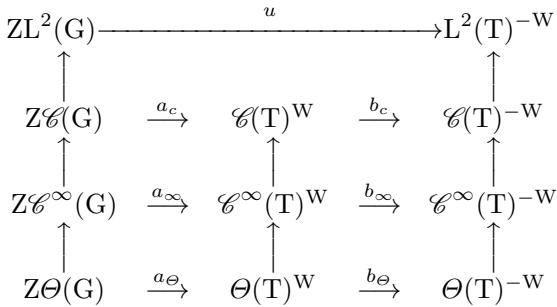
\includegraphics[keepaspectratio]{images/part003_8b0b3ceb.jpg}}

where the vertical arrows are the canonical inclusions, the maps \(b_{c}, b_{\infty}, b_{\Theta}\) are induced by b, and u extends \(b_{c} \circ a_{c}\) by continuity (§7, no. 4, Cor. 3 of Th. 2). The maps u and \(b_{\Theta}\) are bijective (loc. cit.); so is \(b_{\infty}\) (Exerc. 5); on the other hand, \(b_{c}\) is not surjective in general (Exerc. 6).

\section{COMPACT LIE GROUPS OPERATING ON MANIFOLDS}

In this paragraph, X denotes a separated, locally finite dimensional, real manifold of class \(C^{r}\) ( \(1 \leq r \leq \omega\) ).

\subsection{EMBEDDING OF A MANIFOLD IN THE NEIGHBOURHOOD OF A COMPACT SET}

Lemma 1. Let T and T' be two topological spaces, A and A' compact subsets of T and T', respectively, W a neighbourhood of A × A' in T × T'. There exists an open neighbourhood U of A in T and an open neighbourhood U' of A' in T' such that U × U' ⊂ W.

Let \(x \in \mathrm{A}\) ; there exist open subsets \(\mathrm{U}_x\) of \(\mathrm{T}\) and \(\mathrm{U}_x'\) of \(\mathrm{T}'\) such that \(\{x\} \times \mathrm{A}' \subset \mathrm{U}_x \times \mathrm{U}_x' \subset \mathrm{W}\) : indeed, the compact subset \(\{x\} \times \mathrm{A}'\) of \(\mathrm{T} \times \mathrm{T}'\) can be covered by a finite number of open sets contained in \(\mathrm{W}\) , of the form \(\mathrm{U}_i \times \mathrm{U}_i'\) , with \(x \in \mathrm{U}_i\) ; it suffices to take \(\mathrm{U}_x = \bigcap_i \mathrm{U}_i\) and \(\mathrm{U}_x' = \bigcup_i \mathrm{U}_i'\) .

Since A is compact, there exist points \(x_{1},\ldots,x_{m}\) of A such that \(A\subset\bigcup_{i}U_{x_{i}}\) ; put \(U=\bigcup_{i}U_{x_{i}}\) and \(U'=\bigcap_{i}U'_{x_{i}}\) . Then \(A\times A'\subset U\times U'\subset W\) , hence the lemma.

In the remainder of this number, Y denotes a separated manifold of class \(C^{r}\) .

PROPOSITION 1. Let \(\varphi : \mathrm{X} \to \mathrm{Y}\) be a morphism of class \(\mathbf{C}^r\) , A a compact subset of \(\mathrm{X}\) . The following conditions are equivalent:

\begin{enumerate}
\def\labelenumi{(\roman{enumi})}
\item
  The restriction of \(\varphi\) to A is injective, and \(\varphi\) is an immersion at every point of A;
\item
  there exists an open neighbourhood U of A such that \(\varphi\) induces an embedding of U into Y.
\end{enumerate}

When these conditions are satisfied, \(\varphi\) is said to be an embedding in the neighbourhood of A.

We prove that (i) implies (ii), the other implication being clear. Assuming (i), there exists an open neighbourhood V of X containing A such that the restriction of \(\varphi\) to V is an immersion (Differentiable and Analytic Manifolds, Results, 5.7.1). Denote by \(\Gamma\) the set of points \((x,y)\) in \(V \times V\) such that \(\varphi(x) = \varphi(y)\) , and by \(\Delta\) the diagonal in \(V \times V\) . Then \(\Delta\) is an open subset of \(\Gamma\) : indeed, for all \(x \in V\) , there exists an open neighbourhood \(U_x\) of x such that the restriction of \(\varphi\) to \(U_x\) is injective, that is, such that \(\Gamma \cap (\mathrm{U}_x \times \mathrm{U}_x) = \Delta \cap (\mathrm{U}_x \times \mathrm{U}_x)\) .

Since Y is separated, \(\varGamma\) is closed in \(V \times V\) ; consequently the complement W of \(\varGamma - \varDelta\) in \(V \times V\) is open. By assumption, W contains \(A \times A\) ; Lemma 1 implies that there exists an open subset \(U'\) of V containing A such that \(U' \times U' \subset W\) , that is, such that the restriction of \(\varphi\) to \(U'\) is injective. Moreover, there exists an open neighbourhood U of A whose closure is compact and contained in \(U'\) (General Topology, Chap. I, §9, no. 7, Prop. 10). Then \(\varphi\) induces a homeomorphism from \(\overline{U}\) to \(\varphi(\overline{U})\) , and consequently from U to \(\varphi(U)\) ; it follows that the restriction of \(\varphi\) to U is an embedding (Differentiable and Analytic Manifolds, Results, 5.8.3).

PROPOSITION 2. Assume that the manifold Y is paracompact; let A be a subset of X, and let \(\varphi : X \to Y\) be a morphism of class \(C^r\) that induces a homeomorphism from A to \(\varphi(A)\) , and that is étale at every point of A. Then there exists an open neighbourhood U of A such that \(\varphi\) induces an isomorphism from U to an open submanifold of Y.

Restricting X and Y if necessary, we can assume that \(\varphi\) is étale and surjective. Denote by \(\sigma : \varphi(A) \to A\) the inverse homeomorphism of \(\varphi|A\) . Since Y is metrizable (Differentiable and Analytic Manifolds, Results, 5.1.6), \(\varphi(A)\) admits a fundamental system of paracompact neighbourhoods; hence, by General Topology, Chap. XI, there exist an open neighbourhood V of \(\varphi(A)\) in Y and a continuous map \(s : V \to X\) , that coincides with \(\sigma\) on \(\varphi(A)\) and is such that \(\varphi(s(y)) = y\) for all \(y \in V\) . Moreover, s is topologically étale, so \(s(V)\) is an open set U containing A. Then \(\varphi\) induces a homeomorphism \(\varphi'\) from U to V; by Differentiable and Analytic Manifolds, Results, 5.7.8, \(\varphi'\) is an isomorphism.

In the remainder of this number, we assume that \(r \neq \omega\) .

PROPOSITION 3. Let A be a compact subset of X. The set P of morphisms \(\varphi \in \mathcal{C}^{r}(X;Y)\) that are embeddings in the neighbourhood of A is open in \(\mathcal{C}^{r}(X;Y)\) in the topology of compact \(C^{r}\) -convergence ( \(\S\) 6, no. 4).

Clearly, it suffices to prove the proposition for \(r = 1\) .

\begin{enumerate}
\def\labelenumi{\alph{enumi})}
\tightlist
\item
  We show first that the subset J of \(\mathcal{C}^{1}(\mathrm{X};\mathrm{Y})\) consisting of the morphisms that are immersions at every point of A is open. Consider the map \(j_{\mathrm{A}}:\mathcal{C}^{1}(\mathrm{X};\mathrm{Y})\times\mathrm{A}\to\mathrm{J}^{1}(\mathrm{X};\mathrm{Y})\) such that \(j_{\mathrm{A}}(\varphi,x)=j_{x}^{1}(\varphi)\) (Differentiable and Analytic Manifolds, Results, 12.1).
\end{enumerate}

By definition of the topology on \(\mathcal{C}^1 (\mathrm{X};\mathrm{Y})\) , the map \(\tilde{j}_{\mathrm{A}}:\varphi \to j_{\mathrm{A}}(\varphi ,.)\) from \(\mathcal{C}^1 (\mathrm{X};\mathrm{Y})\) to \(\mathcal{C}(\mathrm{A};\mathrm{J}^1 (\mathrm{X};\mathrm{Y}))\) is continuous; it now follows from General Topology, Chap. X, §3, no. 4, Th. 3, that \(j_{\mathrm{A}}\) is continuous.

On the other hand, let M be the set of jets j in \(\mathrm{J}^{1}(\mathrm{X};\mathrm{Y})\) whose tangent map \(\mathrm{T}(j):\mathrm{T}_{\mathbf{s}(j)}(\mathrm{X})\to\mathrm{T}_{\mathbf{b}(j)}(\mathrm{Y})\) (Differentiable and Analytic Manifolds, Results, 12.3.4) is injective. The set M is open in \(\mathrm{J}^{1}(\mathrm{X};\mathrm{Y})\) ; indeed, it suffices to verify this assertion when X is an open subset of a finite dimensional vector space E, and Y is an open subset of a Banach space F; we are then reduced (Differentiable and Analytic Manifolds, Results, 12.3.1) to proving that the set of injective continuous linear maps is open in \(\mathcal{L}(\mathrm{E};\mathrm{F})\) , which follows from Spectral Theory, Chap. III, §2, no. 7, Prop. 16.

We conclude from the preceding that the set \(j_{\mathrm{A}}^{-1}(\mathrm{M})\) is open in \(\mathcal{C}^{1}(\mathrm{X};\mathrm{Y})\times\mathrm{A}\) , hence that its complement F is closed. Since A is compact, the projection \(\mathrm{pr}_{1}:\mathcal{C}^{1}(\mathrm{X};\mathrm{Y})\times\mathrm{A}\to\mathcal{C}^{1}(\mathrm{X};\mathrm{Y})\) is a proper morphism, hence closed; consequently, the set J, which is equal to \(\mathcal{C}^{1}(\mathrm{X};\mathrm{Y})-\mathrm{pr}_{1}(\mathcal{F})\) , is open in \(\mathcal{C}^{1}(\mathrm{X};\mathrm{Y})\) .

\begin{enumerate}
\def\labelenumi{\alph{enumi})}
\setcounter{enumi}{1}
\tightlist
\item
  Let H be the subset of \(J \times A \times A\) consisting of the elements \((f, x, y)\) such that \(f(x) = f(y)\) . It is clear that H contains \(J \times \Delta\) , where \(\Delta\) denotes the diagonal in the product \(A \times A\) ; we show that \(H' = H - (J \times \Delta)\) is closed in \(J \times A \times A\) . Since P is the complement in J of the image of \(H'\) under the proper projection \(pr_{1}: J \times A \times A \to J\) , this will imply the proposition.
\end{enumerate}

The topology of \(\mathcal{C}^{1}(\mathrm{X};\mathrm{Y})\) being finer than the topology of compact convergence, the map \((\varphi,x)\mapsto\varphi(x)\) from \(\mathcal{C}^{1}(\mathrm{X};\mathrm{Y})\times\mathrm{A}\) to Y is continuous (General Topology, Chap. X, §3, no. 4, Cor. 1 of Th. 3); it follows that H is closed in \(J\times A\times A\) . Hence, it suffices to show that \(J\times\Delta\) is open in H, in other words, that for all \(\varphi\in J\) and all \(x\in A\) there exists a neighbourhood \(\Omega\) of \(\varphi\) in J and a neighbourhood B of x in X such that, for any morphism \(\psi\) in \(\Omega\) , the restriction of \(\psi\) to \(A\cap B\) is injective.

Thus, the proposition follows from the following lemma:

Lemma 2. Let x be a point of X, \(\varphi: X \to Y\) a morphism of class \(C^{1}\) that is an immersion at x. There exists a neighbourhood \(\Omega\) of \(\varphi\) in \(\mathcal{C}^{1}(X;Y)\) and a neighbourhood B of x in X such that, for all \(\psi \in \Omega\) , the restriction of \(\psi\) to B is injective.

Let U be a relatively compact open neighbourhood of x isomorphic to a finite dimensional vector space, and such that \(\varphi(\overline{\mathrm{U}})\) is contained in the domain V of a chart. The set \(\Omega_{0}\) of \(\psi\in\mathcal{C}^{1}(\mathrm{X};\mathrm{Y})\) such that \(\psi(\overline{\mathrm{U}})\subset\mathrm{V}\) is open in \(\mathcal{C}^{1}(\mathrm{X};\mathrm{Y})\) , and the restriction map \(\Omega_{0}\to\mathcal{C}^{1}(\mathrm{U};\mathrm{V})\) is continuous; we are thus reduced to proving the lemma when X=U and Y=V, in other words, we can assume that X is a finite dimensional vector space and Y is a Banach space. Choose norms on X and Y.

The linear map \(\mathrm{D}\varphi(x):\mathrm{X}\to\mathrm{Y}\) is injective; denote its conorm by q (Spectral Theory, Chap. III, §2, no. 6), so that, by definition, we have \(\|\mathrm{D}\varphi(x).t\|\geq q\|t\|\) for all \(t\in X\) . Let \(\varepsilon\in R\) be such that \(0<\varepsilon<q/2\) , and let B be a closed ball with centre x such that \(\|\mathrm{D}\varphi(u)-\mathrm{D}\varphi(x)\|\leq\varepsilon\) for all \(u\in B\) . Denote by \(\Omega\) the subset of \(\mathcal{C}^{1}(\mathrm{X};\mathrm{Y})\) consisting of the morphisms \(\psi\) such that \(\|\mathrm{D}\psi(u)-\mathrm{D}\varphi(u)\|\leq\varepsilon\) for all \(u\in B\) ; it is open by definition of the topology of \(\mathcal{C}^{1}(\mathrm{X};\mathrm{Y})\) . For \(\psi\in\Omega\) , put \(\psi_{0}=\psi-\mathrm{D}\varphi(x)\) . We have \(\|\mathrm{D}\psi_{0}(u)\|\leq2\varepsilon\) for all \(u\in B\) , and consequently \(\|\psi_{0}(u)-\psi_{0}(v)\|\leq2\varepsilon\|u-v\|\) for all u and v in B (Differentiable and Analytic Manifolds, Results, 2.2.3). It follows that

\[
\| \psi (u) - \psi (v) \| \geq \| \mathrm{D} \varphi (x). (u - v) \| - \| \psi_ {0} (u) - \psi_ {0} (v) \| \geq (q - 2 \varepsilon) \| u - v \|.
\]

Consequently, the restriction of \(\psi\) to B is injective, hence the lemma.

PROPOSITION 4. Let A be a compact subset of X. There exist a finite dimensional vector space E and a morphism \(\varphi \in \mathcal{C}^r (\mathrm{X};\mathrm{E})\) ( \(r\neq \omega\) ) that is an embedding in the neighbourhood of A.

Let \((\mathrm{U}_{i},\varphi_{i},\mathrm{E}_{i})_{i\in\mathrm{I}}\) be a finite family of charts of X whose domains cover A. We extend \(\varphi_{i}\) to a map from X to \(E_{i}\) (also denoted by \(\varphi_{i}\) ) by putting \(\varphi_{i}(x)=0\) for \(x\notin U_{i}\) . Let \((\mathrm{V}_{i})_{i\in\mathrm{I}}\) be a covering of A by open subsets of X such that \(\overline{\mathrm{V}}_{i}\subset\mathrm{U}_{i}\) for all \(i\in\mathrm{I}\) (the existence of such a covering follows from General Topology, Chap. IX, §4, no. 3, Cor. 1 of Th. 3, applied to the compact space \(X'\) obtained by adjoining to X a point at infinity and the covering of \(X'\) consisting of the open sets \(U_{i}\) ( \(i\in\mathrm{I}\) ) and \(X'-\mathrm{A}\) ). For all \(i\in\mathrm{I}\) , let \(\alpha_{i}\) be a numerical function of class \(C^{r}\) on X, equal to 1 at every point of \(V_{i}\) , and with support contained in \(U_{i}\) (Differentiable and Analytic Manifolds, Results, 5.3.6).

Consider the map \(\varphi : \mathrm{X} \to \bigoplus_{i \in \mathrm{I}} (\mathrm{E}_i \oplus \mathbf{R})\) defined by

\[
\varphi (x) = (\alpha_ {i} (x) \varphi_ {i} (x), \alpha_ {i} (x)) _ {i \in I}.
\]

For all \(i \in I\) , the map \(\alpha_{i}\varphi_{i}\) is of class \(C^{r}\) (since its restrictions to \(U_{i}\) and to the complement of the support of \(\alpha_{i}\) are), and its restriction to \(V_{i}\) is an embedding; it follows that \(\varphi\) is a morphism of class \(C^{r}\) and is an immersion at every point of A. We show that the restriction of \(\varphi\) to A is injective. Let x, y be two points of A such that \(\varphi(x) = \varphi(y)\) , and let \(i \in I\) be such that \(x \in V_{i}\) . Then \(\alpha_{i}(x) = 1\) , so \(\alpha_{i}(y) = 1\) , which implies that \(y \in U_{i}\) ; but we also have \(\varphi_{i}(x) = \varphi_{i}(y)\) , so x = y since \(\varphi_{i}\) induces an embedding of \(U_{i}\) into \(E_{i}\) .

It can be shown \(^{9}\) that every separated manifold, countable at infinity and of pure dimension n, embeds in \(R^{2n}\) ; for a weaker result, cf.~Exercise 2.

\subsection{EQUIVARIANT EMBEDDING THEOREM}

In this number, we assume that \(r \neq \omega\) .

Lemma 3. Let G be a compact topological group operating continuously on a topological space X; let A be a subset of X, stable under G, and W a neighbourhood of A. Then, there exists an open neighbourhood V of A stable under G and contained in W.

Put \(\mathrm{F} = \mathrm{X} - \mathrm{W}\) and \(\mathrm{V} = \mathrm{X} - \mathrm{GF}\) . Then \(\mathrm{V}\) is open (General Topology, Chap. III, §4, no. 1, Cor. 1 of Prop. 1), stable under \(\mathrm{G}\) , and \(\mathrm{A} \subset \mathrm{V} \subset \mathrm{W}\) .

THEOREM 1. Let G be a compact Lie group, \((g,x)\mapsto gx\) a law of left operation of class \(C^{r}\) of G on X, and A a compact subset of X. There exists an analytic linear representation \(\rho\) of G on a finite dimensional vector space E, a morphism \(\varphi:X\to E\) of class \(C^{r}\) , compatible with the operations of G, and an open neighbourhood U of A, stable under G, such that the restriction of \(\varphi\) to U is an embedding.

Replacing A by the compact set GA, we are reduced to the case in which A is stable under G.

Let \(E_0\) be a finite dimensional vector space such that there exists an element of \(\mathcal{C}^r(\mathrm{X};\mathrm{E}_0)\) that is an embedding in the neighbourhood of A (no. 1, Prop. 4); the set \(\mathcal{P}\) of morphisms having this property is a non-empty open subset of \(\mathcal{C}^r(\mathrm{X};\mathrm{E}_0)\) (no. 1, Prop. 3). Consider the continuous linear representation of the compact group G on the space \(\mathcal{C}^r(\mathrm{X};\mathrm{E}_0)\) (§6, no. 4, Lemma 4). By the Peter-Weyl theorem (Spectral Theory, in preparation), the union of the finite dimensional subspaces stable under G is dense in \(\mathcal{C}^r(\mathrm{X};\mathrm{E}_0)\) ; hence, there exists an element \(\varphi_0\) of \(\mathcal{P}\) such that the maps \(x \mapsto \varphi_0(gx)\) , for \(g \in G\) , generate a finite dimensional vector subspace \(E_1\) of \(\mathcal{C}^r(\mathrm{X};\mathrm{E}_0)\) , which is clearly stable under the operation of G.

Take E to be the space \(\operatorname{Hom}_{\mathbf{R}}(\mathrm{E}_{1},\mathrm{E}_{0})\) , \(\rho\) to be the representation of G on E induced by the action on \(E_{1}\) , and \(\varphi:X\to E\) to be the map that associates to \(x\in X\) the linear map \(\psi\mapsto\psi(x)\) from \(E_{1}\) to \(E_{0}\) . This is a morphism of class \(C^{r}\) ; for \(x\in X\) , \(g\in G\) , \(\psi\in E_{1}\) , we have (denoting by \(\tau(g)\) the automorphism \(x\mapsto gx\) of X):

\[
\varphi (g x) (\psi) - \psi (g x) = \varphi (x) (\psi \circ \tau (g)) = (\rho (g) \varphi (x)) (\psi).
\]

Let \(\alpha : \mathrm{Hom}_{\mathbf{R}}(\mathrm{E}_1, \mathrm{E}_0) \to \mathrm{E}_0\) be the linear map \(u \mapsto u(\varphi_0)\) ; we have \(\alpha \circ \varphi = \varphi_0\) , so \(\varphi\) is an embedding in the neighbourhood of A because \(\varphi_0\) is one. Hence, there exists an open neighbourhood U of A such that the restriction of \(\varphi\) to U is an embedding; we can choose U stable under G by Lemma 3, hence the theorem.

COROLLARY 1. Assume that X is compact. There exists an analytic linear representation \(\rho\) of G on a finite dimensional vector space E and an embedding \(\varphi: X \to E\) such that \(\varphi(gx) = \rho(g)\varphi(x)\) for \(g \in G, x \in X\) .

COROLLARY 2. Let H be a closed subgroup of G. There exists an analytic linear representation of G on a finite dimensional vector space E and a point \(v \in E\) with fixer H.

Apply Cor. 1 to the canonical operation of G on the compact manifold G/H. This gives an analytic linear representation \(\rho: \mathrm{G} \to \mathbf{GL}(\mathrm{E})\) and an embedding \(\varphi: \mathrm{G} / \mathrm{H} \to \mathrm{E}\) such that \(\varphi(gx) = \rho(g)\varphi(x)\) , \(g \in \mathrm{G}, x \in \mathrm{G} / \mathrm{H}\) . Let \(\bar{e} \in \mathrm{G} / \mathrm{H}\) be the class of \(e \in \mathrm{G}\) , and \(v = \varphi(\bar{e})\) its image. For all \(g \in \mathrm{G}\) , we have \(\rho(g)v = v \Longleftrightarrow \varphi(g\bar{e}) = \varphi(\bar{e}) \Longleftrightarrow g\bar{e} = \bar{e} \Longleftrightarrow g \in \mathrm{H}\) .

COROLLARY 3. Assume that X is paracompact. There exists a real Hilbert space E, a continuous unitary representation \({}^{10}\) \(\rho\) of G on E and an embedding \(\varphi: X \to E\) of class \(C^{r}\) such that \(\varphi(gx) = \rho(g)\varphi(x)\) for all \(g \in G\) and all \(x \in X\) .

The space X/G is locally compact (General Topology, Chap. III, §4, no. 5, Prop. 11). Its connected components are the images of the connected components of X, which are countable at infinity (General Topology, Chap. I, §9, no. 10, Th. 5); thus, they are themselves countable at infinity, which implies that X/G is paracompact (loc. cit.). Hence, there exists a locally finite covering \((\mathrm{U}_{\alpha}^{\prime})_{\alpha\in\mathrm{I}}\) of X/G by relatively compact open sets, and a covering \((\mathrm{V}_{\alpha}^{\prime})_{\alpha\in\mathrm{I}}\) such that \(\overline{V}_{\alpha}^{\prime}\subset U_{\alpha}^{\prime}\) for all \(\alpha\in I\) (General Topology, Chap. IX, §4, no. 3, Cor. 1 of Th. 3); taking the inverse image, we obtain two locally finite coverings \((\mathrm{U}_{\alpha})_{\alpha\in\mathrm{I}}\) and \((\mathrm{V}_{\alpha})_{\alpha\in\mathrm{I}}\) of X by relatively compact open sets stable under G, such that \(\overline{V}_{\alpha}\subset U_{\alpha}\) for all \(\alpha\in I\) .

For all \(\alpha \in \mathrm{I}\) , there exists a representation \(\rho_{\alpha}\) of G on a finite dimensional real vector space \(\mathrm{E}_{\alpha}\) and a morphism \(\varphi_{\alpha} \in \mathcal{C}^r (\mathrm{X};\mathrm{E}_{\alpha})\) , compatible with the operations of G, whose restriction to \(\mathrm{U}_{\alpha}\) is an embedding (Th. 1). For \(\alpha \in \mathrm{I}\) , let \(a_{\alpha}\) be a numerical function of class \(\mathrm{C}^r\) on X, equal to 1 on \(\mathrm{V}_{\alpha}\) and to 0 outside \(\mathrm{U}_{\alpha}\) (Differentiable and Analytic Manifolds, Results, 5.3.6). Put \(b_{\alpha}(x) = \int_{\mathrm{G}} a_{\alpha}(gx) dg\) for \(x \in \mathrm{X}\) . The function \(b_{\alpha}\) is of class \(\mathrm{C}^r\) , invariant under G (§6, no. 4, Cor. 2), equal to 1 on \(\mathrm{V}_{\alpha}\) and to 0 outside \(\mathrm{U}_{\alpha}\) . Give each \(\mathrm{E}_{\alpha}\) a Hilbert scalar product invariant under G (§1, no. 1), and R its canonical Hilbert structure; let E be the Hilbert sum of the family \((\mathrm{E}_{\alpha} \oplus \mathbf{R})_{\alpha \in \mathrm{I}}\) , and let \(\rho\) be the representation of G on E induced by the \(\rho_{\alpha}\) and the trivial action of G on R. For \(x \in \mathrm{X}\) , put \(\varphi(x) = (b_{\alpha}(x)\varphi_{\alpha}(x), b_{\alpha}(x))_{\alpha \in \mathrm{I}}\) . Then \(\varphi\) is a morphism of class \(\mathrm{C}^r\) from X to E, compatible with the operations of G; we verify as in the proof of Prop. 4 (no. 1) that \(\varphi\) is an embedding, which implies the corollary.

\subsection{TUBES AND TRANSVERSALS}

Lemma 4. Let H be a compact Lie group, \(\rho : \mathrm{H} \to \mathbf{GL}(\mathrm{V})\) a continuous (hence analytic) representation of H on a finite dimensional real vector space, and W a neighbourhood of the origin in V. There exists an open neighbourhood B of the origin, contained in W and stable under H, and an analytic isomorphism \(u: \mathrm{V} \to \mathrm{B}\) , compatible with the operations of H, such that \(u(0) = 0\) and \(\mathrm{Du}(0) = \mathrm{Id}_{\mathrm{V}}\) .

Choose a scalar product on V invariant under H (§1, no. 1). There exists a real number \(r > 0\) such that the open ball B of radius \(r\) is contained in W; it is clearly stable under H. Put \(u(v) = r(r^2 + \|v\|^2)^{-1/2} v\) for all \(v \in V\) ; then \(u\) is a bijective analytic map from V to B, compatible with the operations of H, and its inverse map \(w \mapsto r(r^2 - \|w\|^2)^{-1/2} w\) is analytic. Moreover, \(u(0) = 0\) and \(\mathrm{D}u(0) = \mathrm{Id}_{\mathrm{V}}\) .

PROPOSITION 5. Let H be a compact Lie group, \((h,x)\mapsto hx\) a law of left operation of class \(C^{r}\) of H on X, and x a point of X fixed under the operation of H. Then the group H operates linearly on the vector space \(T=T_{x}(X)\) ; there exists an open embedding \(\varphi:T\to X\) of class \(C^{r}\) , compatible with the operations of H, such that \(\varphi(0)=x\) and \(T_{0}(\varphi)\) is the identity map of T.

Let \((\mathrm{U},\psi,\mathrm{E})\) be a chart of X at x, such that U is stable under H (no. 2, Lemma 3) and such that \(\psi(x)=0\) . Identify E with T by means of \(\mathrm{T}_{x}(\psi)\) , and put

\[
\psi^ {\sharp} (y) = \int_ {\mathrm{H}} h. \psi (h ^ {- 1} y) d h \quad \text { for } y \in \mathrm{U},
\]

where dh is the Haar measure on H of total mass 1.

Then (§6, no. 4, Cor. 1) \(\psi^{\sharp}\) is a morphism of class \(\mathrm{C}^r\) from U to T, compatible with the operations of H, such that \(\psi^{\sharp}(x) = 0\) and \(d_x\psi^\sharp = \mathrm{Id}_\mathrm{T}\) . Hence, there exists an open set \(\mathrm{U}' \subset \mathrm{U}\) containing \(x\) , and an open neighbourhood V of 0 in T, such that \(\psi^{\sharp}\) induces an isomorphism \(\theta: \mathrm{U}' \to \mathrm{V}\) . Restricting \(\mathrm{U}'\) and V if necessary, we can assume that they are stable under H and that there exists an isomorphism \(u: \mathrm{T} \to \mathrm{V}\) compatible with the operations of H (Lemma 4). It now suffices to take \(\varphi = \theta^{-1} \circ u\) .

Recall (Differentiable and Analytic Manifolds, Results, 6.5.1) that if G is a Lie group, H a Lie subgroup of G and Y a manifold on which H operates on the left, we denote by \(G \times^{H}Y\) the quotient of the product manifold \(G \times Y\) by the right operation \(((g,y),h) \mapsto (gh,h^{-1}y)\) of H; this is a manifold on which the Lie group G operates naturally on the left; the projection \(G \times^{H}Y \to G/H\) is a bundle with fibre Y. Further, if Y is a finite dimensional vector space on which H operates linearly, \(G \times^{H}Y\) has a natural structure of vector G-bundle with base G/H (Differentiable and Analytic Manifolds, Results, 7.10.2).

Let G be a Lie group operating properly on the manifold X (General Topology, Chap. III, §4, no. 1, Def. 1) such that the law of operation \((g, x) \mapsto gx\) is of class \(C^{r}\) . Then, for every point x of X, the orbit Gx of x is a closed submanifold of X, isomorphic to the Lie homogeneous space \(G/G_{x}\) , where \(G_{x}\) is the fixer of x in G (cf.~Chap. III, §1, no. 7, Prop. 14 (ii), and General Topology, Chap. III, §4, no. 2, Prop. 4); this is a compact Lie group (loc. cit.).

PROPOSITION 6. Assume that the manifold X is paracompact; let x be a point of X, \(G_{x}\) its fixer. There exists a finite dimensional analytic linear representation \(\tau: G_{x} \to \mathbf{GL}(W)\) , and an open embedding \(\alpha: G \times ^{G_{x}} W \to X\) of class \(C^{r}\) , compatible with the operations of G, that maps the class of \((e,0) \in G \times W\) to x.

Put \(T = T_{x}(X)\) . Let W be a complementary subspace of \(T_{x}(Gx)\) in T, stable under \(G_{x}\) (for example, the orthogonal complement of \(T_{x}(Gx)\) with respect to a scalar product on T invariant under \(G_{x}\) ). On the other hand, let \(\varphi : T \to X\) be a morphism with the properties stated in Prop. 5 (relative to \(H = G_{x}\) ). Consider the morphism \(\lambda : G \times W \to X\) defined by \(\lambda(g, w) = g\varphi(w)\) . It induces by passage to the quotient a morphism \(\mu : G \times^{G_{x}}W \to X\) of class \(C^{r}\) , compatible with the operations of G, that maps the class z of \((e, 0)\) to x.

We show that \(\mu\) is étale at the point \(z\) . We have

\[
\begin{array}{c} \dim (\mathrm{G} \times {} ^ {\mathrm{G} _ {x}} \mathrm{W}) = \dim (\mathrm{G}) + \dim (\mathrm{W}) - \dim (\mathrm{G} _ {x}) \\ = \dim (\mathrm{G} x) + \dim (\mathrm{W}) = \dim (\mathrm{T}), \end{array}
\]

so it suffices to show that \(\mu\) is submersive at \(z\) , or equivalently that \(\lambda\) is submersive at \((e,0)\) . But, the tangent map \(\mathrm{T}_{(e,0)}(\lambda):\mathrm{T}_e(\mathrm{G})\oplus \mathrm{W}\to \mathrm{T}\) is equal to \(\mathrm{T}_e(\rho (x)) + i\) , where \(\rho (x)\) is the orbital map \(g\mapsto gx\) and \(i\) the canonical injection from W to T; since \(\operatorname {Im}\operatorname {T}_e(\rho (x)) = \operatorname {T}_x(\operatorname {G}x)\) , the map \(\mathrm{T}_{(e,0)}(\lambda)\) is surjective, and \(\mu\) is étale at \(z\) .

We are going to show that there exists an open neighbourhood \(\Omega\) of \(Gz\) in \(G \times ^{G_x}W\) , stable under \(G\) , such that \(\mu\) induces an isomorphism from \(\Omega\) onto an open subset of \(X\) . This will imply the proposition: indeed, the inverse image of \(\Omega\) in \(G \times W\) is stable under \(G\) , and hence is of the form \(G \times B\) , where \(B\) is an open subset of \(W\) containing the origin and stable under \(G_x\) ; restricting \(\Omega\) if necessary, we can assume that there exists an isomorphism \(u: W \to B\) , compatible with the operations of \(G_x\) (Lemma 4). It is clear that the composite morphism \(\alpha: G \times ^{G_x}W \xrightarrow{(\text{Id}, u)} G \times ^{G_x}B \xrightarrow{\mu} X\) satisfies the conditions in the statement of the proposition.

Thus, the proposition is a consequence of the following lemma:

Lemma 5. Let Z be a separated manifold of class \(C^{r}\) , equipped with a law of left operation \(m: G \times Z \to Z\) of class \(C^{r}\) , and \(\mu: Z \to X\) a morphism (of class \(C^{r}\) ) compatible with the operations of G. Let z be a point of Z, and \(x = \mu(z)\) . Assume that \(\mu\) is étale at z, and that the fixer of z in G is equal to the fixer \(G_{x}\) of x. Then, there exists an open neighbourhood \(\Omega\) of the orbit Gz, stable under G, such that \(\mu\) induces an isomorphism from \(\Omega\) onto an open subset of X.

Since \(\mu\) is compatible with the operations of G, it is étale at every point of Gz; since the canonical map \(G/G_{x} \rightarrow Gx\) is a homeomorphism, so is the map from Gz to Gx induced by \(\mu\) . Hence, it follows from Prop. 2 of no. 1 that there exists an open neighbourhood U of Gz in Z such that \(\mu\) induces an open embedding of U into X.

Since G operates properly on X, there exists an open neighbourhood V of x and a compact subset K of G such that \(gV \cap V = \varnothing\) for \(g \notin K\) (General Topology, Chap. III, §4, no. 4, Prop. 7); in particular, \(e \in K\) . The set \(W_{1}\) of points \(y \in Z\) such that \(Ky \subset U\) is open in Z: indeed, \(Z - W_{1}\) is the image of the closed set \((\mathrm{K} \times \mathrm{Z}) - m^{-1}(\mathrm{U})\) under the proper projection \(pr_{2}: K \times Z \to Z\) . Put \(W = W_{1} \cap \mu^{-1}(V)\) ; this is an open subset of Z, containing z, and satisfying the following conditions:

\begin{enumerate}
\def\labelenumi{(\roman{enumi})}
\item
  KW \(\subset\) U, and in particular W \(\subset\) U;
\item
  \(\mu(\mathrm{W}) \subset \mathrm{V}.\)
\end{enumerate}

Put \(\Omega = \mathrm{GW}\) and consider the restriction of \(\mu\) to \(\Omega\) . This is an étale morphism, since every point of \(\Omega\) is conjugate under \(\mathbf{G}\) to a point of \(\mathbf{U}\) . We show that it is injective: let \(g, h\) in \(\mathbf{G}\) and \(u, v\) in \(\mathbf{W}\) be such that \(\mu(gu) = \mu(hv)\) . Put \(k = g^{-1}h\) ; then \(\mu(u) = k\mu(v)\) , so \(k \in \mathbf{K}\) by (ii). But \(kv\) and \(u\) belong to \(\mathbf{U}\) by (i); thus, \(u = kv\) because the restriction of \(\mu\) to \(\mathbf{V}\) is injective, so \(gu = hv\) . Hence, the restriction of \(\mu\) to \(\Omega\) is injective, and consequently (Differentiable and Analytic Manifolds, Results, 5.7.8) is an isomorphism onto an open submanifold of \(\mathbf{X}\) , which completes the proof.

Under the conditions of Prop. 6, the image of \(\alpha\) is an open neighbourhood T of the orbit A of \(x\) , equipped with the structure of vector bundle with base A, for which the zero section is the orbit A itself. Such a neighbourhood is called a linear tube (around the orbit in question). For each point \(a \in \mathrm{A}\) , the fibre \(\mathrm{Y}_a\) of this vector bundle is a submanifold of X, stable under the fixer \(\mathrm{G}_a\) of \(a\) , and such that the morphism from \(\mathrm{G} \times^{\mathrm{G}_a}\mathrm{Y}_a\) to X that maps the class of \((g,y) \in \mathrm{G} \times \mathrm{Y}_a\) to \(gy \in \mathrm{X}\) induces a morphism of class \(\mathrm{C}^r\) from \(\mathrm{G} \times^{\mathrm{G}_a}\mathrm{Y}_a\) to T. Then \(\mathrm{Y}_a\) is said to be the transversal at \(a\) of the tube T. We remark that the tangent space at \(a\) of \(\mathrm{Y}_a\) is canonically isomorphic to \(\mathrm{Y}_a\) and that it is a complement of \(\mathrm{T}_a(\mathrm{A})\) in \(\mathrm{T}_a(\mathrm{X})\) ; thus, the vector bundle T with base A is canonically isomorphic to the normal bundle of A in X (Differentiable and Analytic Manifolds, Results, 8.1.3).

\subsection{ORBIT TYPES}

Let \(G\) be a topological group operating continuously on a separated topological space \(E\) . For every point \(x\) of \(E\) , denote by \(G_x\) the fixer of \(x\) in \(G\) , and assume that the canonical map \(G / G_x \to Gx\) is a homeomorphism; this is notably the case in the following two situations:

\begin{enumerate}
\def\labelenumi{\alph{enumi})}
\item
  the topologies of G and E are discrete;
\item
  G operates properly on E (General Topology, Chap. III, §4, no. 2, Prop. 4), for example, G is compact (General Topology, Chap. III, §4, no. 1, Prop. 2).
\end{enumerate}

Denote by \(\mathcal{T}\) the set of conjugacy classes of closed subgroups of G. For every \(x\in \mathrm{E}\) , we call the orbit type of \(x\) , or sometimes the type of \(x\) , the class of \(\mathrm{G}_x\) in \(\mathcal{T}\) ; two points of the same orbit are of the same orbit type (Algebra, Chap. I, §5, no. 2, Prop. 2); two orbits are of the same type if and only if they are isomorphic as G-sets (Algebra, Chap. I, §5, no. 5, Th. 1). For every \(t\in \mathcal{T}\) , denote by \(\mathrm{E}_{(t)}\) the set of points of E of type \(t\) , that is, the union of the orbits of type \(t\) ; this is a stable subset of E. For \(\mathrm{H}\in t\) , we also write \(\mathrm{E}_{(\mathrm{H})}\) for \(\mathrm{E}_{(t)}\) ; for example, \(\mathrm{E}_{(\mathrm{G})}\) is the closed subspace of E consisting of the points fixed by G.

Give T the following preorder relation:

\(t \leq t'\Longleftrightarrow\) there exists \(\mathrm{H} \in t\) and \(\mathrm{H}' \in t'\) such that \(\mathrm{H} \supset \mathrm{H}'\) .

Let \(\Omega\) and \(\Omega'\) be two orbits of G on E, \(t\) and \(t'\) their types; then \(t \leq t'\) if and only if there exists a G-morphism (necessarily surjective and continuous) from \(\Omega'\) to \(\Omega\) .

Let \(x, x'\) be in E, and \(t, t'\) their types; then \(t \leq t'\) if and only if there exists \(a \in G\) such that \(aG_{x'}a^{-1} \subset G_x\) .

Lemma 6. Let G be a Lie group.

\begin{enumerate}
\def\labelenumi{\alph{enumi})}
\item
  Every decreasing sequence of compact subgroups of \(\mathbf{G}\) is stationary.
\item
  Let H and \(H'\) be two compact subgroups of G such that \(H \subset H'\) and such that there exists an isomorphism (of topological groups) from \(H'\) to H. Then \(H = H'\) .
\item
  With the relation \(t \leq t'\) , the set \(\mathcal{T}\) is a noetherian ordered set (Theory of Sets, Chap. III, §6, no. 5, text preceding Prop. 7).
\item
  Let \((\mathrm{H}_{i})_{i\geq1}\) be a decreasing sequence of compact subgroups of G; these are Lie subgroups of G (Chap. III, §8, no. 2, Th. 2). The sequence of integers \((\dim\mathrm{H}_{i})_{i\geq1}\) is decreasing, hence stationary, so there exists an integer N such that the subgroups \(H_{i}\) have the same identity component for \(i\geq N\) . Then the decreasing sequence of positive integers \((\mathrm{H}_{i}:(\mathrm{H}_{i})_{0})_{i\geq N}\) is stationary, so \(H_{i}=H_{i+1}\) for i sufficiently large.
\item
  Let \(f\) be an isomorphism from \(\mathrm{H}'\) to \(\mathrm{H}\) . The sequence \((f^n(\mathrm{H}))_{n\geq 0}\) is a decreasing sequence of compact subgroups of \(\mathrm{G}\) , so \(f^n(\mathrm{H}) = f^{n + 1}(\mathrm{H})\) for \(n\) sufficiently large, by \(a\) ). Since \(f\) is an isomorphism, this implies that \(f(\mathrm{H}) = \mathrm{H} = f(\mathrm{H}')\) , so \(\mathrm{H} = \mathrm{H}'\) .
\item
  Let \(t, t' \in \mathcal{T}\) be such that \(t \leq t'\) and \(t' \leq t\) . Then, there exist \(\mathrm{H}, \mathrm{H}_1 \in t\) and \(\mathrm{H}', \mathrm{H}_1' \in t'\) such that \(\mathrm{H} \supset \mathrm{H}'\) and \(\mathrm{H}_1 \subset \mathrm{H}_1'\) . Let \(g\) and \(g'\) be two elements of \(G\) such that \(\mathrm{H}_1 = g\mathrm{H}g^{-1}\) and \(\mathrm{H}_1' = g'\mathrm{H}'g'^{-1}\) ; put \(u = g'^{-1}g\) . Then
\end{enumerate}

\[
u \mathrm{H} u ^ {- 1} \subset \mathrm{H} ^ {\prime} \subset \mathrm{H};
\]

by \(b\) ), this implies that \(u\mathrm{H}u^{-1} = \mathrm{H}\) , so \(\mathrm{H}' = \mathrm{H}\) and \(t' = t\) . Thus, the set \(\mathcal{T}\) is ordered, and it is noetherian by \(a\) ).

THEOREM 2. Let \(\mathbf{G}\) be a Lie group operating properly on \(\mathbf{X}\) , such that the law of operation \((g,x)\mapsto gx\) is of class \(\mathbf{C}^r\) . Assume that \(\mathbf{X}\) is paracompact.

\begin{enumerate}
\def\labelenumi{\alph{enumi})}
\item
  The map which associates to any point of X its orbit type has the following semi-continuity property: let \(x \in X\) and let \(t \in T\) be its orbit type; there exists a stable open neighbourhood U of x such that, for any \(u \in U\) , the type of u is \(\geq t\) .
\item
  For all \(t \in \mathcal{T}\) , \(\mathrm{X}_{(t)}\) is a submanifold of \(\mathrm{X}\) , the equivalence relation on \(\mathrm{X}_{(t)}\) induced by the operation of \(\mathrm{G}\) is regular (Differentiable and Analytic Manifolds, Results, 5.9.5), and the morphism \(\mathrm{X}_{(t)} \to \mathrm{X}_{(t)} / \mathrm{G}\) is a bundle.
\item
  Assume that X/G is connected. Then the set of orbit types of elements of X has a largest element \(\tau\) ; moreover, \(\mathrm{X}_{(\tau)}\) is a dense open subset of X and \(\mathrm{X}_{(\tau)}/\mathrm{G}\) is connected.
\end{enumerate}

Let \(x\) be a point of \(\mathrm{X}\) and \(t \in \mathcal{T}\) its type. To prove \(a)\) and \(b)\) , we can replace \(\mathrm{X}\) by a stable open set containing \(x\) , and hence (Prop. 6) can assume that \(\mathrm{X}\) is of the form \(\mathrm{G} \times^{\mathrm{H}}\mathrm{W}\) , where \(\mathrm{W}\) is the space of a finite dimensional analytic linear representation of a compact subgroup \(\mathrm{H}\) of \(\mathrm{G}\) , the point \(x\) being the image \(p(e,0)\) of \((e,0) \in \mathrm{G} \times \mathrm{W}\) under the canonical projection \(p: \mathrm{G} \times \mathrm{W} \to \mathrm{G} \times^{\mathrm{H}}\mathrm{W}\) . If \(u = p(g,y) \in \mathrm{G} \times^{\mathrm{H}}\mathrm{W}\) and \(a \in \mathrm{G}\) , then \(au = u\) if and only if there exists \(h \in \mathrm{H}\) with \((ag,y) = (gh^{-1},hy)\) , that is, if \(a \in g\mathrm{H}_yg^{-1}\) . Thus, \(\mathrm{G}_u = g\mathrm{H}_yg^{-1}\) ; in particular, \(\mathrm{G}_x = \mathrm{H}\) , so \(\mathrm{G}_u\) is conjugate to a subgroup of \(\mathrm{G}_x\) , which proves that the type of \(u\) is \(\geq t\) , hence \(a)\) .

Moreover, u is of type t if and only if \(G_{u}\) is conjugate to H in G, or equivalently that \(H_{y}\) is conjugate to H in G; by Lemma 6 b), this means that \(H_{y} = H\) , and hence that y is fixed by H. If \(W'\) is the vector subspace of W consisting of the elements fixed by H, it follows that \(\mathrm{X}_{(t)}\) can be identified with \(G \times {}^{H}W'\) , and hence also with \(G/H \times W'\) , hence b).

To prove c), observe that the assumption that X/G is connected implies that X is pure of finite dimension: indeed, for all \(k \geq 0\) , denote by \(X_{k}\) the set of points \(x \in X\) such that \(\dim_{x} X = k\) ; then \(X_{k}\) is open and closed in X, and stable under G, so X is equal to one of the \(X_{k}\) .

We now prove c) by induction on the dimension of X, the assertion being clear for \(\dim X = 0\) . Let \(\tau\) be a maximal element among the orbit types of the points of X (such an element exists by Lemma 6 c)). We shall prove the following:

\(c^{\prime})\) For every subset A of \(\mathrm{X}_{(t)}\) , open and closed in \(\mathrm{X}_{(\tau)}\) and stable under G, the closure \(\overline{\mathrm{A}}\) of A in X is open.

This assertion implies \(c\) ). Indeed, note first that \(\mathrm{X}_{(\tau)}\) is open in \(\mathrm{X}\) , by \(a\) ; assertion \(c'\) ) implies that \(\overline{\mathrm{X}}_{(\tau)}\) is open and closed in \(\mathrm{X}\) , hence equal to \(\mathrm{X}\) since it is stable under \(\mathrm{G}\) and \(\mathrm{X} / \mathrm{G}\) is connected. Let \(\mathrm{A}\) be a non-empty open and closed subset of \(\mathrm{X}_{(\tau)}\) stable under \(\mathrm{G}\) ; by \(c'\) ), \(\overline{\mathrm{A}}\) is open and closed in \(\mathrm{X}\) and stable under \(\mathrm{G}\) , hence equal to \(\mathrm{X}\) ; this implies that \(\mathrm{A}\) is dense in

\(X_{(\tau)}\) , hence equal to \(X_{(\tau)}\) . Consequently, every non-empty open and closed subset of \(X_{(\tau)}/G\) is equal to \(X_{(\tau)}/G\) , which proves that \(X_{(\tau)}/G\) is connected. Finally, since \(X_{(\tau)}\) is dense in X, it follows from a) that every point of X is of type \(\leq \tau\) ; in other words, \(\tau\) is the largest element among the orbit types of the points of X.

We now prove \(c'\) . We can assume that A is non-empty; let \(x \in \overline{A}\) . It suffices to prove that \(\overline{A}\) is a neighbourhood of x. For this we can, as above, assume that \(X = G \times {}^{H}W\) with H compact, x being the canonical image of \((e,0)\) . Assume first that H operates trivially on W: then X can be identified with \((G/H) \times W\) , and \(X_{(\tau)}/G = X/G\) is homeomorphic to W, hence connected; thus, A/G = X/G, so A = X. Assume from now on that H does not operate trivially on W. Choose a scalar product on W invariant under the compact group H; let S be the unit sphere in W (the set of vectors of norm 1). Note that S/H is connected: indeed, if \(\dim(W) \geq 2\) , S is connected, and if \(\dim(W) = 1\) , S is a space of two points on which H operates non-trivially. Put \(Y = G \times {}^{H}S\) ; this is a closed submanifold of X, stable under G, of codimension 1, and Y/G, which is homeomorphic to S/H, is connected. Thus, by the induction hypothesis, there exists a maximal orbit type \(\theta\) for Y, the set \(Y_{(\theta)}\) is open and dense in Y, and \(Y_{(\theta)}/G\) is connected.

Consider the operation of \(R_{+}^{*}\) on X induced by passage to the quotient by the law of operation \((\lambda, (g, w)) \mapsto (g, \lambda w)\) of \(R_{+}^{*}\) on G × W. Two points of X conjugate under this operation are of the same orbit type; consequently, \(\mathrm{X}_{(\theta)}\) contains \(\mathbf{R}_{+}^{*}\mathrm{Y}_{(\theta)}\) , which is a dense open subset of X. But \(\mathrm{X}_{(\tau)}\) is open by a), and hence meets \(\mathrm{X}_{(\theta)}\) , so \(\theta = \tau\) .

On the other hand, the homeomorphism \((\lambda,w)\mapsto\lambda w\) from \(R_{+}^{*}\times S\) to \(W-\{0\}\) (General Topology, Chap. VI, §2, no. 3, Prop. 3) induces a homeomorphism from \(R_{+}^{*}\times(S/H)\) to \((\mathbf{R}_{+}^{*}\mathrm{S})/\mathrm{H}\) , hence also from \(R_{+}^{*}\times(Y/G)\) to \((\mathbf{R}_{+}^{*}\mathrm{Y})/\mathrm{G}\) , and from \(R_{+}^{*}\times(\mathrm{Y}_{(\theta)}/\mathrm{G})\) to \((\mathbf{R}_{+}^{*}\mathrm{Y}_{(\theta)})/\mathrm{G}\) . Thus, \((\mathbf{R}_{+}^{*}\mathrm{Y}_{(\theta)})/\mathrm{G}\) is connected, and \(X_{(\tau)}/\mathrm{G}\) , which contains a connected dense subset, is itself connected (General Topology, Chap. I, §11, no. 1, Prop. 1). Consequently, A is equal to \(X_{(\tau)}\) , hence is dense in X, and \(\overline{A}\) is a neighbourhood of x. This completes the proof of the theorem.

With the notations in Th. 2 c), the points of \(\mathrm{X}_{(\tau)}\) are said to be principal and their orbits are called principal orbits. If x is a point of X, and if \(G \times G_{x}W\) is a linear tube in X around the orbit of x, the point x is principal if and only if \(G_{x}\) operates trivially on W, that is, if the tube is of the form \((\mathrm{G}/\mathrm{G}_{x}) \times \mathrm{W}\) .

Examples. 1) Let G be a connected compact Lie group, operating on itself by inner automorphisms. The fixer of an element x of G is simply the centralizer \(Z(x)\) of x in G; it contains every maximal torus containing x. It follows that the largest orbit type \(\tau\) is the conjugacy class of the maximal tori of G. The open set \(\mathrm{G}_{(\tau)}\) is the set of very regular elements of G ( \(\S5\) , no. 1, Remark). Assume that G is simply-connected. Then \(\mathrm{G}_{(\tau)}\) is equal to the set \(G_{r}\) of regular elements of G ( \(\S5\) , no. 2, Remark 2); if A is an alcove of a Cartan subalgebra t of \(\mathfrak{g} = \mathrm{L}(\mathrm{G})\) , the composite map \(\pi: A \xrightarrow{\exp} G_{r} \longrightarrow G_{r}/\mathrm{Int}(\mathrm{G})\) is an isomorphism of analytic manifolds. Indeed, this is a homeomorphism (§5, no. 2, Cor. of Prop. 2); let \(a \in A\) , put \(t = \exp a\) and identify \(T_{t}(\mathrm{G})\) with g by means of the translation \(\gamma(t)\) . The tangent map \(T_{a}(\pi)\) can then be identified with the composite of the canonical injection \(t \to g\) and the quotient map \(g \to g/\mathrm{Im}(\mathrm{Ad} t^{-1} - 1)\) . Since t is regular, \(T_{a}(\pi)\) is an isomorphism, hence the stated result (Differentiable and Analytic Manifolds, Results, 5.7.8).

\begin{enumerate}
\def\labelenumi{\arabic{enumi})}
\setcounter{enumi}{1}
\tightlist
\item
  Let E be a real euclidean affine space, H a set of hyperplanes of E, W the group of displacements of E generated by the orthogonal reflections with respect to the hyperplanes of H. Assume that H is stable under W and that the group W, with the discrete topology, operates properly on E.
\end{enumerate}

The preceding can be applied to the operation of W on E. The fixer of a point x of E is the subgroup of W generated by the reflections with respect to the hyperplanes of H containing x (Chap. V, §3, no. 3, Prop. 2). Consequently, the largest orbit type \(\tau\) is the class of the subgroup \(\{Id_{E}\}\) , and \(\mathrm{E}_{(\tau)}\) is the union of the chambers of E. Note that in this case the covering \(\mathrm{E}_{(\tau)} \to \mathrm{E}_{(\tau)}/\mathrm{W}\) is trivial, and in particular \(\mathrm{E}_{(\tau)}\) is not connected if H is non-empty.

\appendixsection{STRUCTURE OF COMPACT GROUPS}

\appendixitem{EMBEDDING A COMPACT GROUP IN A PRODUCT OF LIE GROUPS}

PROPOSITION 1. Every compact topological group G is isomorphic to a closed subgroup of a product of compact Lie groups.

Denote by \(\hat{\mathbf{G}}\) the set of classes of irreducible continuous unitary representations of \(\mathbf{G}\) on finite dimensional complex Hilbert spaces (Spectral Theory, in preparation). For all \(u\in \hat{\mathbf{G}}\) , let \(\mathrm{H}_u\) be the space of \(u\) and \(\rho_{u}:\mathbf{G}\to \mathbf{U}(\mathrm{H}_{u})\) the homomorphism associated to \(u\) . By the Peter-Weyl theorem (Spectral Theory, in preparation), the continuous homomorphism \(\rho = (\rho_u)_{u\in \hat{\mathbf{G}}}\) from \(\mathbf{G}\) to \(\prod_{u\in \hat{\mathbf{G}}}\mathbf{U}(\mathrm{H}_u)\) is injective; since \(\mathbf{G}\) is compact, \(\rho\) induces an isomorphism from \(\mathbf{G}\) onto a closed subgroup of the group \(\prod_{\hat{\mathbf{G}}} \mathbf{U}(\mathrm{H}_u)\) .
COROLLARY 1. Let V be a neighbourhood of the identity element of G. Then V contains a closed normal subgroup H of G such that the quotient G/H is a Lie group.

Let \((\mathrm{K}_{\lambda})_{\lambda \in \mathrm{L}}\) be a family of compact Lie groups such that \(\mathrm{G}\) can be identified with a closed subgroup of \(\prod_{\lambda \in \mathrm{L}}\mathrm{K}_{\lambda}\) ; for \(\lambda \in \mathrm{L}\) , demote by \(p_{\lambda}:\mathrm{G}\to \mathrm{K}_{\lambda}\) the restriction to G of the canonical projection. There exists a finite subset \(J \subset L\) , and for each \(\lambda \in J\) a neighbourhood \(V_{\lambda}\) of the origin in \(K_{\lambda}\) , such that V contains \(\bigcap_{\lambda \in J} p_{\lambda}^{-1}(V_{\lambda})\) . It now suffices to put \(H = \bigcap_{\lambda \in J} \text{Ker}(p_{\lambda})\) .

Denote by \((\mathrm{H}_{\alpha})_{\alpha\in\mathrm{I}}\) the decreasing filtered family of closed normal subgroups of G, such that the quotient \(G/H_{\alpha}\) is a Lie group. Consider the projective system of compact Lie groups \(G/H_{\alpha}\) (cf.~General Topology, Chap. III, §7, no. 2, Prop. 2).

COROLLARY 2. The canonical map \(\mathrm{G} \to \varprojlim_{\alpha} \mathrm{G} / \mathrm{H}_{\alpha}\) is an isomorphism of topological groups.

Indeed, Cor. 1 implies that condition (PA) of General Topology, Chap. III, §7, no. 2, is satisfied; the assertion now follows from Prop. 2 of loc. cit.

COROLLARY 3. G is a Lie group if and only if there exists a neighbourhood of the identity element e of G that contains no normal subgroup distinct from \(\{e\}\) .

The necessity of this condition has already been proved (Chap. III, §4, no. 2, Cor. 1 of Th. 2), and the sufficiency is an immediate consequence of Cor. 1.

\appendixitem{PROJECTIVE LIMITS OF LIE GROUPS}

Lemma 1. Let \((\mathrm{G}_{\alpha}, f_{\alpha \beta})\) be a projective system of topological groups relative to a filtered index set I, and G its limit. Assume that the canonical maps \(f_{\alpha}: \mathrm{G} \to \mathrm{G}_{\alpha}\) are surjective.

\begin{enumerate}
\def\labelenumi{\alph{enumi})}
\item
  The subgroups \(\overline{\mathrm{D}(\mathrm{G}_{\alpha})}\) (resp. \(\mathrm{C}(\mathrm{G}_{\alpha})\) , resp. \(\mathrm{C}(\mathrm{G}_{\alpha})_0\) ) form a projective system of subsets of \(\mathrm{G}_{\alpha}\) .
\item
  We have \(\overline{\mathrm{D}(\mathrm{G})}=\varprojlim_{\alpha}\overline{\mathrm{D}(\mathrm{G}_{\alpha})}\) and \(\mathrm{C}(\mathrm{G})=\varprojlim_{\alpha}\mathrm{C}(\mathrm{G}_{\alpha})\) .
\item
  If \(\mathrm{G}_{\alpha}\) is compact for all \(\alpha \in \mathrm{I}\) , then \(\mathrm{C}(\mathrm{G})_0 = \varprojlim_{\alpha} \mathrm{C}(\mathrm{G}_{\alpha})_0\) .
\end{enumerate}

Let \(\alpha, \beta\) be two elements of I, with \(\alpha \leq \beta\) . Then \(f_{\alpha \beta}(\mathrm{D}(\mathrm{G}_{\beta})) \subset \mathrm{D}(\mathrm{G}_{\alpha})\) , and \(f_{\alpha \beta}(\mathrm{C}(\mathrm{G}_{\beta})) \subset \mathrm{C}(\mathrm{G}_{\alpha})\) since \(f_{\alpha \beta}\) is surjective; since \(f_{\alpha \beta}\) is continuous, it follows that \(f_{\alpha \beta}(\overline{\mathrm{D}(\mathrm{G}_{\beta})}) \subset \overline{\mathrm{D}(\mathrm{G}_{\alpha})}\) and \(f_{\alpha \beta}(\mathrm{C}(\mathrm{G}_{\beta})_0) \subset \mathrm{C}(\mathrm{G}_{\alpha})_0\) , hence \(a)\) . Since \(f_{\alpha}\) is surjective, \(f_{\alpha}(\mathrm{D}(\mathrm{G})) = \mathrm{D}(\mathrm{G}_{\alpha})\) (Algebra, Chap. I, §6, no. 2, Prop. 6), so \(\overline{\mathrm{D}(\mathrm{G})} = \varprojlim \overline{\mathrm{D}(\mathrm{G}_{\alpha})}\) (General Topology, Chap. I, §4, no. 4, Cor. of Prop. 9). The surjectivity of \(f_{\alpha}\) also implies the inclusion \(f_{\alpha}(\mathrm{C}(\mathrm{G})) \subset \mathrm{C}(\mathrm{G}_{\alpha})\) and hence \(\mathrm{C}(\mathrm{G}) \subset \varprojlim \mathrm{C}(\mathrm{G}_{\alpha})\) ; the opposite inclusion is immediate. Finally, assertion \(c)\) follows from \(b)\) and General Topology, Chap. III, §7, no. 2, Prop. 4).

Lemma 2. Let \((\mathrm{S}_a)_{a\in \mathrm{A}},(\mathrm{T}_b)_{b\in \mathrm{B}}\) be two finite families of almost simple, simply-connected Lie groups (Chap. III, § 9, no. 8, Def. 3), \(u:\prod_{a\in \mathrm{A}}\mathrm{S}_a\to \prod_{b\in \mathrm{B}}\mathrm{T}_b\) a surjective morphism. Then there exist an injective map \(l: \mathrm{B} \to \mathrm{A}\) and isomorphisms \(u_b: \mathrm{S}_{l(b)} \to \mathrm{T}_b\) ( \(b \in \mathrm{B}\) ) such that \(u((s_a)_{a \in \mathrm{A}}) = (u_b(s_{l(b)}))_{b \in \mathrm{B}}\) for every element \((s_a)_{a \in \mathrm{A}}\) of \(\prod_{a \in \mathrm{A}} \mathrm{S}_a\) .

Denote by \(\mathfrak{s}_a\) (resp. \(\mathfrak{t}_b\) ) the Lie algebra of \(S_a\) (resp. \(T_b\) ) for \(a \in A\) (resp. \(b \in B\) ), and consider the homomorphism \(L(u): \prod_{a \in A} \mathfrak{s}_a \to \prod_{b \in B} \mathfrak{t}_b\) . Its kernel is an ideal of the semi-simple Lie algebra \(\prod_{a \in A} \mathfrak{s}_a\) , and hence is of the form \(\prod_{a \in A''} \mathfrak{s}_a\) , with \(A'' \subset A\) (Chap. I, §6, no. 2, Cor. 1). Put \(A' = A - A''\) . By restriction, \(L(u)\) induces an isomorphism \(f: \prod_{a \in A'} \mathfrak{s}_a \to \prod_{b \in B} \mathfrak{t}_b\) . By loc. cit., for all \(a \in A'\) the ideal \(f(\mathfrak{s}_a)\) is equal to one of the \(\mathfrak{t}_b\) ; hence, there exists a bijection \(l: B \to A'\) such that \(f(\mathfrak{s}_{l(b)}) = \mathfrak{t}_b\) for \(b \in B\) , and \(f\) induces an isomorphism \(f_b: \mathfrak{s}_{l(b)} \to \mathfrak{t}_b\) . Since the groups \(S_a\) and \(T_b\) are simply-connected, there exist isomorphisms \(u_b: S_{l(b)} \to T_b\) such that \(L(u_b) = f_b\) for \(b \in B\) (Chap. III, §6, no. 3, Th. 3).

Denote by \(\tilde{u}:\prod_{a\in \mathrm{A}}\mathrm{S}_a\to \prod_{b\in \mathrm{B}}\mathrm{T}_b\) the morphism defined by \(\tilde{u} ((s_a)_{a\in \mathrm{A}}) = (u_b(s_{l(b)}))_{b\in \mathrm{B}}\) . By construction, \(\mathrm{L}(\tilde{u}) = f = \mathrm{L}(u)\) , so \(\tilde{u} = u\) , which proves the lemma.

Lemma 3. Under the hypotheses of Lemma 1, assume that the \(G_{\alpha}\) are simply-connected compact Lie groups. Then, the topological group G is isomorphic to the product of a family of almost simple, simply-connected compact Lie groups.

For all \(\alpha \in \mathrm{I}\) , the group \(\mathrm{G}_{\alpha}\) is the direct product of a finite family of almost simple, simply-connected subgroups \((\mathrm{S}_{\alpha}^{\lambda})_{\lambda \in \mathrm{L}_{\alpha}}\) (Chap. III, §9, no. 8, Prop. 28). Let \(\beta \in \mathrm{I}\) , \(\beta \geq \alpha\) . By Lemma 2, there exists a map \(l_{\beta \alpha}: \mathrm{L}_{\alpha} \to \mathrm{L}_{\beta}\) such that \(f_{\alpha \beta}(\mathrm{S}_{\beta}^{l_{\beta \alpha}(\lambda)}) = \mathrm{S}_{\alpha}^{\lambda}\) for \(\lambda \in \mathrm{L}_{\alpha}\) . We have \(l_{\gamma \beta} \circ l_{\beta \alpha} = l_{\gamma \alpha}\) for \(\alpha \leq \beta \leq \gamma\) , so \((\mathrm{L}_{\alpha}, l_{\beta \alpha})\) is an inductive system of sets relative to I. Let L be its limit; the maps \(l_{\beta \alpha}\) being injective, \(\mathrm{L}_{\alpha}\) can be identified with a subset of L, so that \(\mathrm{L} = \bigcup_{\alpha \in \mathrm{I}} \mathrm{L}_{\alpha}\) .

Let \(\lambda \in L\) . Put \(S_{\alpha}^{\lambda} = \{1\}\) when \(\lambda \notin L_{\alpha}\) , and denote by \(\varphi_{\alpha \beta}^{\lambda}: S_{\beta}^{\lambda} \to S_{\alpha}^{\lambda}\) the morphism induced by \(f_{\alpha \beta}\) ; this gives a projective system of topological groups \((S_{\alpha}^{\lambda}, \varphi_{\alpha \beta}^{\lambda})\) , whose limit is isomorphic to \(S_{\lambda}\) . The canonical homomorphism of topological groups

\[
\lim_{\substack{\longleftarrow \\ \alpha \in I}}\left(\prod_{\lambda \in L}S_{\alpha}^{\lambda}\right)\to \prod_{\lambda \in L}\left(\lim_{\substack{\longleftarrow \\ \alpha \in I}}S_{\alpha}^{\lambda}\right)
\]

is bijective (Theory of Sets, Chap. III, §7, no. 3, Cor. 2); it is thus an isomorphism since the groups in question are compact. But the first of these groups can be identified with G and the second with the product of the \(S_{\lambda}\) , hence the lemma.

\appendixitem{STRUCTURE OF CONNECTED COMPACT GROUPS}

Let G be a commutative compact group. Recall (Spectral Theory, Chap. II, §1, no. 9, Prop. 11) that G is then isomorphic to the dual topological group of a discrete commutative group \(\hat{G}\) . The group G is connected if and only if \(\hat{G}\) is torsion-free (Spectral Theory, Chap. II, §2, no. 2, Cor. 1 of Prop. 4).

The following properties are equivalent (Spectral Theory, Chap. II, §2, no. 2, Cor. 2 of Prop. 4 and §1, no. 9, Cor. 2 of Prop. 11):

\begin{enumerate}
\def\labelenumi{(\roman{enumi})}
\item
  G is totally discontinuous;
\item
  \(\hat{\mathrm{G}}\) is a torsion group;
\item
  the topological group G is isomorphic to the limit of a projective system of finite (commutative) groups, each having the discrete topology.
\end{enumerate}

The proposition below generalizes Cor. 1 of Prop. 4 of §1, no. 4.

PROPOSITION 2. Let G be a connected compact group.

\begin{enumerate}
\def\labelenumi{\alph{enumi})}
\item
  \(\mathrm{C}(\mathrm{G})_{0}\) is a commutative connected compact group; \(\mathrm{D}(\mathrm{G})\) is a connected compact group, equal to its derived group.
\item
  The continuous homomorphism \((x,y)\mapsto xy\) from \(\mathrm{C}(\mathrm{G})_{0}\times\mathrm{D}(\mathrm{G})\) to G is surjective and its kernel is a central subgroup of \(\mathrm{C}(\mathrm{G})_{0}\times\mathrm{D}(\mathrm{G})\) that is compact and totally discontinuous.
\item
  There exists a family \((\mathrm{S}_{\lambda})_{\lambda\in\mathrm{L}}\) of almost simple compact Lie groups and a surjective continuous homomorphism \(\prod_{\lambda\in\mathrm{L}}\mathrm{S}_{\lambda}\to\mathrm{D}(\mathrm{G})\) , whose kernel is a totally discontinuous, compact, central subgroup.
\end{enumerate}

Let \((\mathrm{G}_{\alpha}, f_{\alpha\beta})\) be a projective system of compact Lie groups, relative to a filtered set I, such that G is isomorphic to \(\varprojlim G_{\alpha}\) and such that the canonical maps \(f_{\alpha}: G \to G_{\alpha}\) are surjective (Cor. 2 of Prop. 1). For \(\alpha \in I\) , let \(\pi_{\alpha}: \tilde{\mathrm{D}}(\mathrm{G}_{\alpha}) \to \mathrm{D}(\mathrm{G}_{\alpha})\) be a universal covering of the group \(\mathrm{D}(\mathrm{G}_{\alpha})\) . The \(f_{\alpha\beta}\) induce morphisms \(\tilde{f}_{\alpha\beta}: \tilde{\mathrm{D}}(\mathrm{G}_{\beta}) \to \tilde{\mathrm{D}}(\mathrm{G}_{\alpha})\) , and \((\tilde{\mathrm{D}}(\mathrm{G}_{\alpha}), \tilde{f}_{\alpha\beta})\) is a projective system of topological groups satisfying the hypotheses of Lemma 3.

It follows from this lemma that the topological group \(\varprojlim\tilde{\mathrm{D}}(\mathrm{G}_{\alpha})\) is isomorphic to the product of a family \((\mathrm{S}_{\lambda})_{\lambda\in\mathrm{L}}\) of almost simple compact Lie groups. By Lemma 1, the limit of the projective system of homomorphisms \((\pi_{\alpha})\) can be identified with a continuous homomorphism \(\pi:\prod_{\lambda\in\mathrm{L}}\mathrm{S}_{\lambda}\to\overline{\mathrm{D}(\mathrm{G})}\) , which is surjective (General Topology, Chap. I, §9, no. 6, Cor. 2 of Prop. 8).

Now observe that the group
\[
\prod_ {\lambda \in L} S _ {\lambda}
\]

is equal to its derived group: this follows from §4, no. 5, Cor. of Prop. 10. The same is true for \(\overline{\mathrm{D(G)}}\) , since \(\pi\) is surjective. Consequently, \(\mathrm{D(G)} \supset \mathrm{D}(\overline{\mathrm{D(G)}}) = \overline{\mathrm{D(G)}}\) . Thus, the group \(\mathrm{D(G)}\) is compact and equal to its derived group; this proves \(a\) ), since the assertions concerning \(\mathrm{C(G)}_0\) are trivial.

On the other hand, the kernel of \(\pi : \prod_{\lambda \in L} S_{\lambda} \to D(G)\) can be identified with \(\varprojlim \operatorname{Ker}(\pi_{\alpha})\) (Algebra, Chap. II, §6, no. 1, Remark 1), and thus with a compact, totally discontinuous, central subgroup, hence \(c\) ).

We prove \(b\) ). For all \(\alpha\) in I, the morphism \(s_{\alpha}: \mathrm{C}(\mathrm{G}_{\alpha})_0 \times \mathrm{D}(\mathrm{G}_{\alpha}) \to \mathrm{G}_{\alpha}\) such that \(s_{\alpha}(x,y) = xy\) for \(x \in \mathrm{C}(\mathrm{G}_{\alpha})_0, y \in \mathrm{D}(\mathrm{G}_{\alpha})\) , is surjective and its kernel is a finite central subgroup (§1, no. 4, Cor. 1 of Prop. 4). The \(s_{\alpha}\) form a projective system of maps, whose limit can, by the preceding, be identified with the homomorphism \((x,y) \mapsto xy\) from \(\mathrm{C}(\mathrm{G})_0 \times \mathrm{D}(\mathrm{G})\) to \(\mathrm{G}\) . We now see as before that this map is surjective and that its kernel is central and totally discontinuous, hence \(b\) ).

COROLLARY. Every solvable connected compact group is commutative.

Indeed, the derived group is then solvable and equal to its derived group (Prop. 2 a)), hence reduced to the identity element.

\appendixsection{REPRESENTATIONS OF REAL, COMPLEX OR QUATERNIONIC TYPE}

\appendixitem{REPRESENTATIONS OF REAL ALGEBRAS}

Denote by \(\sigma\) the automorphism \(\alpha\mapsto\bar{\alpha}\) of C; if W is a complex vector space, denote by \(\overline{W}\) the C-vector space \(\sigma_{*}(W)\) (that is, the group W with the law of operation \((\alpha,w)\mapsto\bar{\alpha}w\) for \(\alpha\in C, w\in W\) ).

PROPOSITION 1. Let A be an R-algebra (associative and unital) and V a finite dimensional simple A-module over R. Then, we must be in one of the following three situations:

\(\alpha)\) The commutant of V (Algebra, Chap. VIII, § 5, no. 1) is isomorphic to \(\mathbf{R}\) , and the \(\mathrm{A}_{(\mathbf{C})}\) -module \(\mathrm{V}_{(\mathbf{C})}\) is simple;

\(\beta)\) the commutant of V is isomorphic to \(\mathbf{C}\) ; the \(\mathrm{A}_{(\mathbf{C})}\) -module \(\mathrm{V}_{(\mathbf{C})}\) is the direct sum of two non-isomorphic simple \(\mathrm{A}_{(\mathbf{C})}\) -submodules which are interchanged by \(\sigma \otimes 1_{\mathrm{V}}\) ;

\(\gamma)\) the commutant of V is isomorphic to H; the \(A_{(C)}\) -module \(V_{(C)}\) is the direct sum of two isomorphic simple \(A_{(C)}\) -submodules that are interchanged by \(\sigma \otimes 1_V\) .

The commutant E of V is a field, a finite extension of R (Algebra, Chap. VIII, §3, no. 2, Prop. 2), hence isomorphic to R, C or H (Algebra, Chap. VIII, §15). The \(A_{(C)}\) -module \(V_{(C)}\) is semi-simple (Algebra, Chap. VIII, §11, no. 4), and its commutant can be identified with \(C \otimes_{R} E\) (Algebra, Chap. VIII, §11, no. 2, Lemma 1).

If \(\mathbf{E}\) is isomorphic to \(\mathbf{R}\) , the commutant of \(V_{(\mathbf{C})}\) is isomorphic to \(\mathbf{C}\) , and \(V_{(\mathbf{C})}\) is a simple \(A_{(\mathbf{C})}\) -module (Algebra, Chap. VIII, §11, no. 4).

If \(\mathbf{E}\) is not isomorphic to \(\mathbf{R}\) , it contains a field isomorphic to \(\mathbf{C}\) ; it follows that \(V\) has an \(A_{(\mathbf{C})}\) -module structure, denoted by \(V^c\) . Then \(V^c\) is a simple

\(A_{(C)}\) -module, and the C-linear map \(\psi: V_{(C)} \to V^{c} \oplus \overline{V}^{c}\) such that \(\psi(\alpha \otimes v) = (\alpha v, \bar{\alpha} v)\) for \(\alpha \in C\) , \(v \in V\) , is an isomorphism (Algebra, Chap. V, §10, no. 4, Prop. 8). Moreover, \(\sigma \otimes 1_{V}\) corresponds under this isomorphism to the R-automorphism \((v, v') \mapsto (v', v)\) of \(V^{c} \oplus \overline{V}^{c}\) , and hence interchanges the two \(A_{(C)}\) -submodules \(\psi^{-1}(V^{c})\) and \(\psi^{-1}(\overline{V}^{c})\) .

The commutant \(E_{(\mathbf{C})}\) of \(V_{(\mathbf{C})}\) thus contains \(C \times C\) , operating by homotheties on \(V^{c} \oplus \overline{V}^{c}\) . There is no isomorphism of \(A_{(\mathbf{C})}\) -modules from \(V^{c}\) to \(\overline{V}^{c}\) if and only if \(E_{(\mathbf{C})}\) reduces to \(C \times C\) , that is, if E is isomorphic to C. This completes the proof.

PROPOSITION 2. Let A be an R-algebra (associative and unital), and W a finite dimensional simple \(\mathrm{A}_{(\mathbf{C})}\) -module over C. Then, we must be in one of the following three situations:

\begin{enumerate}
\def\labelenumi{\alph{enumi})}
\item
  There exists an \(A_{(\mathbf{C})}\) -isomorphism \(\theta\) from W to \(\overline{W}\) with \(\theta \circ \theta = 1_{W}\) . Then the set V of fixed points of \(\theta\) is an R-structure on W, and a simple A-module with commutant R.1 \(_{V}\) . Moreover, \(W_{[R]}\) is the direct sum of two isomorphic simple A-modules.
\item
  The \(\mathrm{A}_{(\mathbf{C})}\) -modules W and \(\overline{\mathrm{W}}\) are not isomorphic; then \(\mathrm{W}_{[\mathbf{R}]}\) is a simple A-module with commutant \(\mathbf{C}.1_{\mathrm{W}}\) .
\item
  There exists an \(\mathrm{A}_{(\mathbf{C})}\) -isomorphism \(\theta\) from W to \(\overline{W}\) with \(\theta \circ \theta = -1_{W}\) . Then the A-module \(W_{[R]}\) is simple, and its commutant is the field \(C.1_{W} \oplus C.\theta\) , which is isomorphic to H.
\end{enumerate}

The complex vector space \(\mathrm{Hom}_{\mathrm{A}_{(\mathbf{C})}}(\mathrm{W},\overline{\mathrm{W}})\) is of dimension \(\leq 1\) (Algebra, Chap. VIII, §3, no. 2); if \(\theta \in \mathrm{Hom}_{\mathrm{A}_{(\mathbf{C})}}(\mathrm{W},\overline{\mathrm{W}})\) , the endomorphism \(\theta \circ \theta\) of W is a homothety, with ratio \(\alpha \in \mathbf{C}\) . For all \(w \in \mathrm{W}\) , we have \(\alpha \theta(w) = \theta \circ \theta \circ \theta(w) = \theta(\alpha w) = \bar{\alpha} \theta(w)\) , so \(\alpha\) is real. If \(\theta' = \lambda \theta\) , with \(\lambda \in \mathbf{C}\) , then \(\theta' \circ \theta' = |\lambda|^2 \theta \circ \theta\) ; thus, exactly one of the following three possibilities is realised:

\begin{enumerate}
\def\labelenumi{\alph{enumi})}
\item
  There exists \(\theta \in \mathrm{Hom}_{\mathrm{A}_{(\mathbf{C})}}(\mathrm{W},\overline{\overline{\mathrm{W}}})\) with \(\theta \circ \theta = 1_{\mathrm{W}}\) ;
\item
  \(\mathrm{Hom}_{\mathrm{A}_{(\mathbf{C})}}(\mathrm{W},\overline{\mathrm{W}}) = \{0\}\) ;
\item
  There exists \(\theta \in \mathrm{Hom}_{\mathrm{A}_{(\mathbf{C})}}(\mathrm{W},\overline{\mathrm{W}})\) with \(\theta \circ \theta = -1_{\mathrm{W}}\) .
\end{enumerate}

In case a), the set V of fixed points of \(\theta\) is an R-structure on W (Algebra, Chap. V, p.~61, Prop. 7); since \(V_{(\mathbf{C})}\) is isomorphic to W, the A-module V is simple with commutant \(R.1_{V}\) (Prop. 1), and \(W_{[R]}\) is not simple.

Conversely, if \(W_{[R]}\) is not simple, let V be a simple A-submodule of \(W_{[R]}\) ; since the \(A_{(C)}\) -module W is simple, \(V + iV = W\) and \(V \cap iV = \{0\}\) , that is, \(W = V \oplus iV\) . Thus, V is an R-structure on W, and the isomorphism \(\theta\) from W to \(\overline{W}\) such that \(\theta(v + iv') = v - iv'\) for v and \(v'\) in V satisfies \(\theta \circ \theta = 1_{W}\) .

Consequently, in cases \(b)\) and \(c)\) , the A-module \(\mathrm{W}_{[\mathbf{R}]}\) is simple; by Prop. 1, its commutant E is isomorphic to C in case \(b)\) , and to H in case \(c)\) . Moreover, it is clear that E contains \(\mathbf{C}.1_{\mathrm{W}}\) , and \(\mathbf{C}.\theta\) in case \(c)\) , hence the proposition.

With the assumptions in the proposition, the \(A_{(C)}\) -module W is said to be of real, complex or quaternionic type (relative to A) in case a), b) or c), respectively.

For K = R or C, denote by \(\mathfrak{S}_{\mathrm{K}}(\mathrm{A})\) the set of classes of finite dimensional simple \(A_{(K)}\) -modules over K. The group \(\Gamma = \operatorname{Gal}(\mathbf{C}/\mathbf{R})\) operates on \(\mathfrak{S}_{\mathbf{C}}(\mathrm{A})\) ; the two preceding propositions establish a bijective correspondence between \(\mathfrak{S}_{\mathbf{R}}(\mathrm{A})\) and the quotient set \(\mathfrak{S}_{\mathbf{C}}(\mathrm{A})/\Gamma\) .